	%!TEX root = ./main.tex

%\documentclass[11pt, a4paper, titlepage, slovak]{book}
\documentclass[12pt, a4paper, titlepage, slovak]{book}

%Includes all neccessary packets and contains some useful commands
%!TEX root = ./main.tex

%----------------------------------------------------------------------------------
%Packages and parameters
%----------------------------------------------------------------------------------

%inputencoding for the mac
%\documentclass[slovak]{article}
\usepackage[T1]{fontenc}
\usepackage[utf8]{inputenc}
\usepackage{babel}

% =========== OLD SETTINGS =========== %
%\usepackage[utf8]{inputenc}
%\usepackage[slovak,english]{babel}
% ================================== %

%packages for mathematical symbols
\usepackage{latexsym}
\usepackage{amsmath}
\usepackage{mathtools}
\usepackage{amssymb}

\usepackage{pdfpages}

% removes 'chapter' word from titles and apply own style
\usepackage{titlesec}
\titleformat{\chapter}{\normalfont\huge\bf}{\thechapter.}{20pt}{\huge\bf}

%table design
\usepackage{booktabs}

%grahics package
\usepackage{color,graphicx}

%path to your image folder
\graphicspath{{images/}}
\usepackage{float} % package for floating images in text

%do not indent at new paragraphs but add a vertical offset
\usepackage{noindent}

%change standard fonts to Palatino and Helvetica
\usepackage{helvet}

%bibliography settings
\usepackage{natbib}
\bibliographystyle{apalike} %harvad style
%\bibliographystyle{ieeepes}

% pdfpages for IIT.SRC paper
\usepackage{pdfpages}

%source code listings
\usepackage{color}
\usepackage{xcolor}
\usepackage{listings}
\usepackage{caption}
\DeclareCaptionFont{white}{\color{white}}
\DeclareCaptionFormat{listing}{\colorbox{gray}{\parbox{\textwidth}{#1#2#3}}}
\captionsetup[lstlisting]{format=listing,labelfont=white,textfont=white}
\renewcommand{\lstlistingname}{Algoritmus}

\lstdefinelanguage{JavaScript}{
keywords={typeof, new, true, false, catch, function, return, null, catch, switch, var, if, in, while, do, else, case, break, let, then},
keywordstyle=\color{blue}\bfseries,
ndkeywords={class, export, boolean, throw, implements, import, this},
ndkeywordstyle=\color{darkgray}\bfseries,
identifierstyle=\color{black},
sensitive=false,
comment=[l]{//},
morecomment=[s]{/*}{*/},
commentstyle=\color{purple}\ttfamily,
stringstyle=\color{red}\ttfamily,
morestring=[b]',
morestring=[b]",
frame=single
}

\lstset{
language=JavaScript,
extendedchars=true,
basicstyle=\footnotesize\ttfamily,
showstringspaces=false,
showspaces=false,
numbers=left,
numberstyle=\footnotesize,
numbersep=9pt,
tabsize=2,
breaklines=true,
showtabs=false,
captionpos=b
}

\lstdefinelanguage{JSON}{
}

\lstset{
	language=JSON,
    string=[s]{"}{"},
    stringstyle=\color{blue},
    comment=[l]{:},
    commentstyle=\color{black},
}

%highlits
\usepackage{framed}
\definecolor{shadecolor}{rgb}{0.75,0.75,0.75}

%citation commands
\newcommand{\fullcite}{\citep} %for "Author [1980]"
\renewcommand{\citeyear}{\citeyearpar} %for "[1980]"

\usepackage{setspace}
%\doublespacing
\onehalfspacing

\usepackage[linesnumbered,ruled]{algorithm2e}

% change images numbering to per subsection
%\usepackage{chngcntr}
%\counterwithin{figure}{section}
%\counterwithin{table}{section}


%package for control structures
\usepackage{ifthen}

%marginpar hack --- moves margin notes to correct position
\usepackage{mparhack}

%make readable references
\usepackage[pdftex,plainpages=false,pdfpagelabels]{hyperref}

% appendix
\usepackage{etoolbox}
\usepackage{lipsum}
\usepackage[titletoc]{appendix}


%---------------------<Layout in the style of "A Pattern Approach to Interaction Design>---------------------------

% Change page headers and footers:
\usepackage{fancyhdr}
\pagestyle{fancy}
\fancyhf{}
\fancyhead[RE]{\slshape \nouppercase{\leftmark}}    % Even page header: "page   chapter"
\fancyhead[LO]{\slshape \nouppercase{\rightmark}}   % Odd  page header: "section   page"
\fancyhead[RO,LE]{\bfseries \thepage} 
\renewcommand{\headrulewidth}{1pt}    % Underline headers
\renewcommand{\footrulewidth}{0pt}    

\fancypagestyle{plain}{               % No chapter+section on chapter start pages
\fancyhf{}
\fancyhead[RO,LE]{\bfseries \thepage}
\renewcommand{\headrulewidth}{1pt}
\renewcommand{\footrulewidth}{0pt}
}

% Left headings: "1  INTRODUCTION"
\renewcommand{\chaptermark}[1]{%
\markboth{\thechapter\ \ \ \ #1}{}}

% Right headings: "1.1  Basics"
\renewcommand{\sectionmark}[1]{%
\markright{\thesection\ \ \ \ #1}{}}


% ZMENA TABULKA ======
\renewcommand{\tablename}{Tabuľka}

% some Fancyhdr problem...
\addtolength{\headheight}{2pt} % To avoid overfull vboxes from fancyhdr

%creating a better way to change the layout for the abstract pages
\usepackage{geometry}

\titlespacing*{\chapter}{0pt}{0pt}{25pt}

% MATUS: change paragraph line spracing
\setlength{\parskip}{0.5em}

\ifthenelse{\lengthtest{\paperheight=250mm}}%
{% -----------------B5 Layout-----------------
% Page layout

%\pdfpageheight250mm
%\pdfpagewidth176mm
\geometry{	b5paper,
			top = 27mm,
			footskip = 10mm,
			inner = 19mm,
			outer = 39mm,
			textheight = 175mm,
			textwidth = 84mm,
			marginparsep = 3mm,
			marginparwidth = 32mm
}
\savegeometry{myText}
% -----------------/ B5 Layout-----------------
}%
{% -----------------A4 Layout-----------------
% Page layout
\geometry{	a4paper,
			twoside,
			includemp,
			includehead,
			top = 20mm,
			headsep = 10mm,
			bindingoffset = 0mm,
			inner = 40mm,
			outer = 30mm,
			bottom = 30mm,
			marginparsep = 0mm,
			marginparwidth = 0mm
}
\savegeometry{myText}
% -----------------/ A4 Layout-----------------
}
% Abstract layout
\geometry{	marginparsep = 0mm,
			marginparwidth = 0mm
}
\savegeometry{myAbstract}
\loadgeometry{myText}


\newlength{\fullwidth} % Width of text plus margin notes
\setlength{\fullwidth}{\textwidth}
\addtolength{\fullwidth}{\marginparsep}
\addtolength{\fullwidth}{\marginparwidth}

\setlength{\headwidth}{\fullwidth} % Header stretches over margin notes


%---------------------</Layout in the style of "A Pattern Approach to Interaction Design>---------------------------


%wird fŸr die flŠchendeckende Ausgabe der Titelseite benštigt
%needed for the full-face titlepage
\usepackage{eso-pic}

%index verwenden
%make an index
\usepackage{makeidx}
\makeindex

%Index Formatierungshilfen
%formatting helpers for the index
\newcommand{\uu}[1]{\underline{#1}}
\newcommand{\ii}[1]{\textit{#1}}

%neue Definition der Index Umgebung
%redesign of the index
\renewenvironment{theindex}{%
  \vspace*{50pt}%
  {\Huge\bfseries\indexname}\par%
  \vspace*{40pt}%
  \setlength{\parskip}{0pt}%
  \setlength{\parindent}{0pt}%
  \small%
  \renewcommand{\item}{\par{}}%
  \renewcommand{\subitem}{\par\hspace{2em}- }%
}%
{}

%Maximale Gliederungstiefe, die noch ins Inhaltsverzeichnis aufgenommen wird
%maximum depth for the table of contents
\setcounter{tocdepth}{3}

%Vorschlag fŸr ein schšnes Farbschema
%Set of colors which look nice together
\usepackage{color}
\definecolor{orange_light}{rgb}{1,0.8,0.4}
\definecolor{orange_med}{rgb}{0.753,0.62,0.373}
\definecolor{orange_dark}{rgb}{0.506,0.412,0.251}

\definecolor{green_light}{rgb}{0.8,1,0.4}
\definecolor{green_med}{rgb}{0.635,0.745,0.376}
\definecolor{green_dark}{rgb}{0.435,0.498,0.255}

\definecolor{blue_light}{rgb}{0.4,0.8,1}
\definecolor{blue_med}{rgb}{0.365,0.624,0.749}
\definecolor{blue_dark}{rgb}{0.251,0.42,0.502}

\definecolor{pink_light}{rgb}{1,0.435,0.812}
\definecolor{pink_med}{rgb}{0.745,0.38,0.62}
\definecolor{pink_dark}{rgb}{0.498,0.255,0.416}

\definecolor{yellow_light}{rgb}{1,1,0.4}
\definecolor{yellow_med}{rgb}{0.757,0.745,0.373}
\definecolor{yellow_dark}{rgb}{0.506,0.49,0.251}

%blau (fŸr URLs)
%blue (for URLs)
\definecolor{blue}{rgb}{0,0,1}

%notwendig fŸr die korrekte Erkennung, auf welcher Seite sich eine Abbildung befindet.
%we need this to determine if a figure is on an odd or even page
\usepackage{chngpage}

%Hiermit kšnnen die Abbildungslegenden frei gestaltet werden
%we need this to redesign the captions
\usepackage[font=normalsize,labelfont=bf]{caption}

%Abbildungen kommen auf eine eigene Seite, wenn sie mehr als 85% des Platzes
%auf einer Seite einnehmen
%if a figure takes more than 85% of a page it will be typeset on a separate page
\renewcommand{\floatpagefraction}{0.85}

%Benštigt um gro§e Abbildungen gedreht auf eine Seite zu setzen
%we need this to rotate big figures
\usepackage[figuresright]{rotating}

%Verschiedene LŠngenma§e fŸr Textboxen
%dimensions for textboxes
\newlength{\myDefBoxWidth}
\setlength{\myDefBoxWidth}{\textwidth}
\addtolength{\myDefBoxWidth}{-4mm}
\newlength{\myBigDefBoxWidth}
\setlength{\myBigDefBoxWidth}{\fullwidth}
\addtolength{\myBigDefBoxWidth}{-4mm}

%Formathilfen fŸr MatLab Code (wer's braucht...)
%pre-defined matlab code formats
\usepackage{alltt}
\definecolor{string}{rgb}{0.7,0.0,0.0}
\definecolor{comment}{rgb}{0.13,0.54,0.13}
\definecolor{keyword}{rgb}{0.0,0.0,1.0}



%-----------------------------------------------------------------------------------------------------------------------------------------
% neue Befehle
% new commands
%-----------------------------------------------------------------------------------------------------------------------------------------

%----------------------------------------------------------------------------------

% \myBigFigure	[ LABEL_PREFIX (optional) ]
%				{ FILENAME (without extension) }
%				{ CAPTION TEXT }
%				{ SHORT VERSION OF CAPTION TEXT }
%
%Bild wird in kompletter Breite gesetzt
%picture using full width of the page
\newcommand{\myBigFigure}[4][image]
{%
\begin{figure}[ht!bp]%
%\begin{figure}[H]%
	\renewcommand{\figurename}{Obrázok}
	\checkoddpage%
	\ifcpoddpage%
		%nothing
	\else
		\hspace{-\marginparsep}\hspace{-\marginparwidth}%
	\fi
	%use minipage to center the label beneath the figure
	\begin{minipage}{\fullwidth}%
		\includegraphics[width= \fullwidth]{#2}%
		\caption[#4]{#3}%
		\label{#1_#2}%
	\end{minipage}%
\end{figure}%
}


%----------------------------------------------------------------------------------
% \myFrameBigFigure	[ LABEL_PREFIX (optional) ]
%					{ FILENAME (without extension) }
%					{ CAPTION TEXT }
%					{ SHORT VERSION OF CAPTION TEXT }
%
%Bild wird in kompletter Breite gesetzt und eingerahmt
%picture with frame using the full width of the page
\newcommand{\myFrameBigFigure}[4][image]
{
\begin{figure}[ht!bp]
%\begin{figure}[H]
	\renewcommand{\figurename}{Obrázok}
	\checkoddpage
	\ifcpoddpage
		%nothing
	\else
		\hspace{-\marginparsep}\hspace{-\marginparwidth}
	\fi
	%use minipage to center the label beneath the figure
	\begin{minipage}{\fullwidth}
	\frame{%
		\includegraphics[width= \fullwidth]{#2}%
		}
		\caption[#4]{#3}
		\label{#1_#2}
	\end{minipage}
\end{figure}
}

%----------------------------------------------------------------------------------
% \myHUGEFigure	[ LABEL_PREFIX (optional) ]
%				{ FILENAME (without extension) }
%				{ CAPTION TEXT }
%				{ SHORT VERSION OF CAPTION TEXT }
%
%Bild wird rotiert und quer in kompletter Breite gesetzt
%landscape picture using the full width of the rotated page
\newcommand{\myHugeFigure}[4][image]
{
\begin{sidewaysfigure}[t!bp]
	\checkoddpage
	\ifcpoddpage
		%nothing
		\vspace{\marginparsep}\vspace{\marginparwidth}
	\else
		%nothing
		\vspace{-\marginparsep}\vspace{-\marginparwidth}
	\fi
		\includegraphics[width= \textheight]{#2}
		\caption[#4]{#3}
		\label{#1_#2}
	
\end{sidewaysfigure}
}

%----------------------------------------------------------------------------------
% \myFigure	[ LABEL_PREFIX (optional) ]
%			{ FILENAME (without extension) }
%			{ CAPTION TEXT }
%			{ SHORT VERSION OF CAPTION TEXT }
%
%Bild wird in der Breite der textspalte gesetzt
%picture using the width of the text column
\newcommand{\myFigure}[6][image]%
{%
%\scalebox{0.5}{
\begin{figure}[#6]%
	\renewcommand{\figurename}{Obrázok}
	\begin{center}%
		\includegraphics[scale=#5]{#2}%
		\caption[#4]{#3}
		\label{#1_#2}%
	\end{center}%
\end{figure}%
}%


%----------------------------------------------------------------------------------
% \myImgRef	[ LABEL_PREFIX (optional) ]
%			{ LABEL OF THE IMAGE }
%
%referenziert das angegebene Bild
%reference to an image
\newcommand{\myImgRef}[2][image]%
{%
	\ref{#1_#2}%
}%

%----------------------------------------------------------------------------------
% \myBigTable	{ YOUR TABULAR DEFINITION }
%			{ CAPTION TEXT }
%			{ TABLE_LABLE }
%
%Tabelle wird in kompletter Breite gesetzt
%table using the full width of the page
\newcommand{\myBigTable}[3]%
{%
\begin{table}[htdp]%
	\checkoddpage%
	\ifcpoddpage%
		%nothing
	\else%
		\hspace{-\marginparsep}\hspace{-\marginparwidth}%
	\fi%
	\begin{minipage}{\fullwidth}%
		\begin{center}%
			#1%
			\caption{#2}%
			\label{#3}%
		\end{center}%	
	\end{minipage}%
\end{table}%
}%

%----------------------------------------------------------------------------------
% \myTable	{ YOUR TABULAR DEFINITION }
%			{ CAPTION TEXT }
%			{ TABLE_LABLE }
%
%Tabelle wird in der Breite der Textspalte gesetzt
%table using the width of the text column
\newcommand{\myTable}[3]%
{%
\begin{table}[htdp]%
	\begin{center}%
		#1%
		\caption{#2}%
		\label{#3}%
	\end{center}%	
\end{table}%
}%

%----------------------------------------------------------------------------------
% \myTxtRef	{ LABLE }
%
%Referenz auf Kapitel oder Abschnitte - gibt nummer und namen aus, z.B.: 5.3---"Yaddahyaddah"
%references chapters or sections, outputs number and title, e.g., 5.3---"Yaddahyaddah"
\newcommand{\myTxtRef}[1]
{%
	\ref{#1} ``\nameref{#1}''%
}

%----------------------------------------------------------------------------------
% \myTxtRefPP	{ LABLE }
%
%Referenz auf Kapitel oder Abschnitte - gibt nummer, namen und seiten aus, z.B.: 5.3---"Yaddahyaddah" (p. 45)
%references chapters or sections, outputs number and title, e.g., 5.3---"Yaddahyaddah"
\newcommand{\myTxtRefPP}[1]
{%
	\ref{#1} ``\nameref{#1}'' (p.~\pageref{#1})%
}

%----------------------------------------------------------------------------------
% \myUnderscore
%
%Setzt einen "schšnen" Unterstrich fŸr URLs
%typesets a 'nice' underscore for URLs
\newcommand{\myUnderscore}{$\underline{\hspace{0.5em}}$}

%----------------------------------------------------------------------------------
%\myTilde
%
%Setzt eine "schšne" Tilde fŸr URLs
%typesets a 'nice' tilde for URLs
\newcommand{\myTilde}{$\sim$}

%----------------------------------------------------------------------------------
% \myURL	{ TYPESET VERSION OF ANCHOR }
%			{ PRISTINE URL }
%			{ TYPESET VERSION OF URL }
%
%Setzt eine URL
%die typographisch "schšne" version erscheint in einer Fu§note,
%im Text erscheint der Ankertext, verlinkt ist die "echte" URL
%typesets a URL
%the typographically correct version appears as a footnote,
%the anchor appears in the text, the link points to the pristine URL
\newcommand{\myURL}[3]%
{%
	\textcolor{blue}{%
		\href{#2}{#1}%
	}%
	\footnote{#3}%
}

%----------------------------------------------------------------------------------
% \mySimpleURL	{ TYPESET VERSION OF ANCHOR }
%				{ PRISTINE URL }
%
%Setzt eine URL
%die URL erscheint in einer Fu§note,
%im Text erscheint der Ankertext, die URL ist verlinkt
%typesets a URL
%the URL appears as a footnote,
%the anchor appears in the text, the link points to the URL
\newcommand{\mySimpleURL}[2]%
{%
	\textcolor{blue}{%
		\href{#2}{#1}%
	}%
	\footnote{#2}%
}

%----------------------------------------------------------------------------------
% \myProjectURL	{ TYPESET VERSION OF ANCHOR }
%				{ PRISTINE URL INSIDE PROJECT DIRECTORY }
%				{ TYPESET VERSION OF URL INSIDE PROJECT DIRECTORY }
%
%Setzt eine URL auf hci/public wo die Inhalte des WebServer Ordners auf "oliver" verfŸgbar sind
%die typographisch "schšne" version erscheint in einer Fu§note,
%im Text erscheint der Ankertext, verlinkt ist die "echte" URL
%typesets a URL to hci/public from where the contents of the WebServer folder from oliver can be accessed
%the typographically correct version appears as a footnote,
%the anchor appears in the text, the link points to the pristine URL
\newcommand{\myProjectURL}[3]%
{%
	\textcolor{blue}{%
		\href{http://hci.rwth-aachen.de/public/#2}{#1}%
	}%
	\footnote{http://hci.rwth-aachen.de/public/#3}%
}

%----------------------------------------------------------------------------------
% \mnote	{ MARGIN NOTE }
%
%Setzt eine Randnotitz
%puts a comment into the margin in small sans-serif font
\newcommand{\mnote}[1]%
{%
	\leavevmode%
	\checkoddpage%
	\ifcpoddpage%
		\marginpar{\raggedright\textsf{{\footnotesize{#1}}}}%
	\else%
		\marginpar{\raggedleft\textsf{{\footnotesize{#1}}}}%
	\fi%
}
	
% leavevmode allows mnotes to be aligned with the first line of a paragraph
% NOTE: you have to put a "%" at the end of the line with the mnote, or you will get an extra blank at the beginning of the paragraph!

%----------------------------------------------------------------------------------
% \todo	{ TODO MARGIN NOTE }
%
%Setzt eine "ToDo"-Randnotitz in rot zur Erinnerung
%puts a 'todo' comment into the margin in red
\definecolor{red}{rgb}{1,0,0}
\newcommand{\todo}[1]{\mnote{\textcolor{red}{ToDo: #1}}}

%----------------------------------------------------------------------------------
% \chapterquote	{ QUOTATION }
%				{ SOURCE }
%
%Setzt ein Zitat zum Einleiten eines Kapitels
%outputs a quote with its source, can be used as an introduction to chapters
\newcommand{\chapterquote}[2]{
\begin{quotation}
    \begin{flushright}
	\noindent\emph{``{#1}''\\[1.5ex]---{#2}}
    \end{flushright}
\end{quotation}
}

%----------------------------------------------------------------------------------
% \myDefBox	{ TERM }
%			{ DEFINITION }
%
%Setzt eine Randnotitz und eine farbige Box (Textspaltenbreite),
%welche einen Begriff und seine Definition enthŠlt
%outputs a margin note and a colored box (width of the text column) containing a term and its definition
\newcommand{\myDefBox}[2]
{%
	\setlength{\fboxrule}{1mm}%
	\fcolorbox{orange_med}{orange_light}%
	{%
		\parbox{\myDefBoxWidth}{{\bfseries\scshape#1:}\\#2}%
	}%
	\mnote{Definition:\\\emph{#1}}
}

%----------------------------------------------------------------------------------
% \myBigDefBox	{ TERM }
%				{ DEFINITION }
%
%Setzt eine farbige Box (Seitenbreite), welche einen Begriff und seine Definition enthŠlt
%outputs a colored box (width of the page) containing a term and its definition
\newcommand{\myBigDefBox}[2]
{%
	\begin{figure}[h!]
	\setlength{\fboxrule}{1mm}%
	\checkoddpage%
	\ifcpoddpage%
		%nothing
	\else%
		\hspace{-\marginparsep}\hspace{-\marginparwidth}%
	\fi%
	\fcolorbox{orange_med}{orange_light}%
	{%
		\parbox{\myBigDefBoxWidth}{{\bfseries\scshape#1:}\\#2}%
	}%
	\end{figure}
}

%----------------------------------------------------------------------------------
% \myDownloadURL	{ TYPESET DOWNLOAD NAME }
%					{ PRISTINE VERSION OF FILENAME }
%					{ TYPESET VERSION OF FILENAME }
%
%Setzt eine farbige Box, welche einen Downloadlink enthŠlt
%outputs a colored box containing a download link
\newcommand{\myDownloadURL}[3]{%
\checkoddpage%
	\ifcpoddpage%
		%nothing
	\else%
		\hspace{-\marginparsep}\hspace{-\marginparwidth}%
	\fi%
\setlength{\fboxrule}{1mm}%
\fcolorbox{green_med}{green_light}{%
\begin{minipage}{\myBigDefBoxWidth}%
\begin{center}%
\myProjectURL{#1}{folder/#2}{folder/#3}%
\end{center}%
\end{minipage}%
}%
}

%----------------------------------------------------------------------------------
% \emptydoublepage
%
% Leere Doppelseite ohne Kopf- oder Fu§zeile am Ende von Kapiteln
% Clear double page without any header or footer at end of chapters
\newcommand{\emptydoublepage}{\clearpage\thispagestyle{empty}\cleardoublepage}
\newcommand{\emptysinglepage}{\clearpage\thispagestyle{empty}\clearpage}

%----------------------------------------------------------------------------------
% \pagebreak	[ SOME STRANGE LATEX VALUE ]
%
%Eklige pagebreaks fŸr den Druck (falls es nicht mehr anders geht)
%pagebreaks for the final print version (last resort weapon against wrong pagebreaks by LaTeX)
\newcommand{\PB}[1][3]
{%
	\pagebreak[#1]%
}

%----------------------------------------------------------------------------------
% \TM
%
%Setzt ein (TM) Symbol
%Places a (TM) symbol
\newcommand{\TM}
{%
	\textsuperscript{\texttrademark}%
}


% zalamovanie slov
\hyphenation{
Twitter
Twittru
map-reduce
oblastiach
korpusov
processing
modelu
vstupno
ZeroMQ
tieto
priamo
vtedy
používateľom
udalostí
}


%--------------------------------------------------------------
\begin{document}

% allow more flexible whitespaces to avoid hyphenation and overfull hboxes
\sloppy %lepsi algoritmus na zalamovanie riadkov

% 'see'-entries for the index
%!TEX root = ./main.tex
%
% This file is part of the i10 thesis template developed and used by the
% Media Computing Group at RWTH Aachen University.
% The current version of this template can be obtained at
% <http://www.media.informatik.rwth-aachen.de/karrer.html>.

\index{abbrv|see{abbreviation}}




%--------------------------------------------------------------
% uvodne strany... obal, titulka, abstrakt, uvod, ...
%--------------------------------------------------------------
\frontmatter

%use the titlepage from the 'images' directory 
\newgeometry{rmargin=20mm}
\begin{titlepage}
% centrovanie
\begin{center}                                                                                                                                                   
{\Large Slovenská technická univerzita v Bratislave} \\
{\Large Fakulta informatiky a informačných technológií} \\
\vspace*{1\baselineskip}
% cislo prace
\large {}
\vfill % vert. plnenie prazdnymi medzerami                                                                                                                                                                    

%\newpage

{{Bc. Matúš Cimerman}} \\
\vspace*{1\baselineskip}
{\LARGE {\textbf{Analýza prúdu prichádzajúcich udalostí použitím rôznych metód pre analýzu údajov}}} % nadpis
%{\huge {Analýza prúdu údajov}} % nadpis
\\
\vspace*{1\baselineskip}
%{\Large {Bakalárska práca}}\\
\textit{Diplomová práca}\\
\vfill %vert. plnenie
\end{center}
% end centrovanie
{Vedúci práce: Ing. Jakub Ševcech, PhD.}\\
\\
%\vspace*{1\baselineskip}
{december, 2016}
\end{titlepage}
\emptydoublepage

\begin{titlepage}
% centrovanie
\begin{center}                                                                                                                                                   
{\Large Slovenská technická univerzita v Bratislave} \\
{\Large Fakulta informatiky a informačných technológií} \\
\vspace*{1\baselineskip}
% cislo prace
\large {}
\vfill % vert. plnenie prazdnymi medzerami                                                                                                                                                                    


{{Bc. Matúš Cimerman}} \\
\vspace*{1\baselineskip}
{\LARGE {\textbf{Analýza prúdu prichádzajúcich udalostí použitím rôznych metód pre analýzu údajov}}} % nadpis
%{\huge {Analýza prúdu údajov}} % nadpis
\\
\vspace*{1\baselineskip}
%{\Large {Bakalárska práca}}\\
\textit{Diplomová práca}\\
\vfill %vert. plnenie
\end{center}
% end centrovanie
{Študijný program: Informačné systémy}\\
{Študijný odbor: 9.2.6 Informačné systémy}\\
{Miesto vypracovania: Ústav informatiky, informačných systémov a softvérového inžinierstva, FIIT STU v Bratislave}\\
{Vedúci práce: Ing. Jakub Ševcech, PhD.}\\
\\
{december, 2016}

\end{titlepage}
\restoregeometry
\thispagestyle{empty}
\emptydoublepage

%% This file is part of the i10 thesis template developed and used by the
% Media Computing Group at RWTH Aachen University.
% The current version of this template can be obtained at
% <http://www.media.informatik.rwth-aachen.de/karrer.html>.

~
\vfill
I hereby declare that I have created this work completely on my own and used no other sources or tools than the ones listed, and that I have marked any citations accordingly.

\begin{flushright}
\vspace{12mm}
$\overline{Bratislava, MONTH \mathit{YEAR}}$\\
\textit{YOUR NAME}
\end{flushright}

%\emptydoublepage

%pred abstrakt treba zadanie
\includepdf[pages={1}]{navrh_1.pdf}
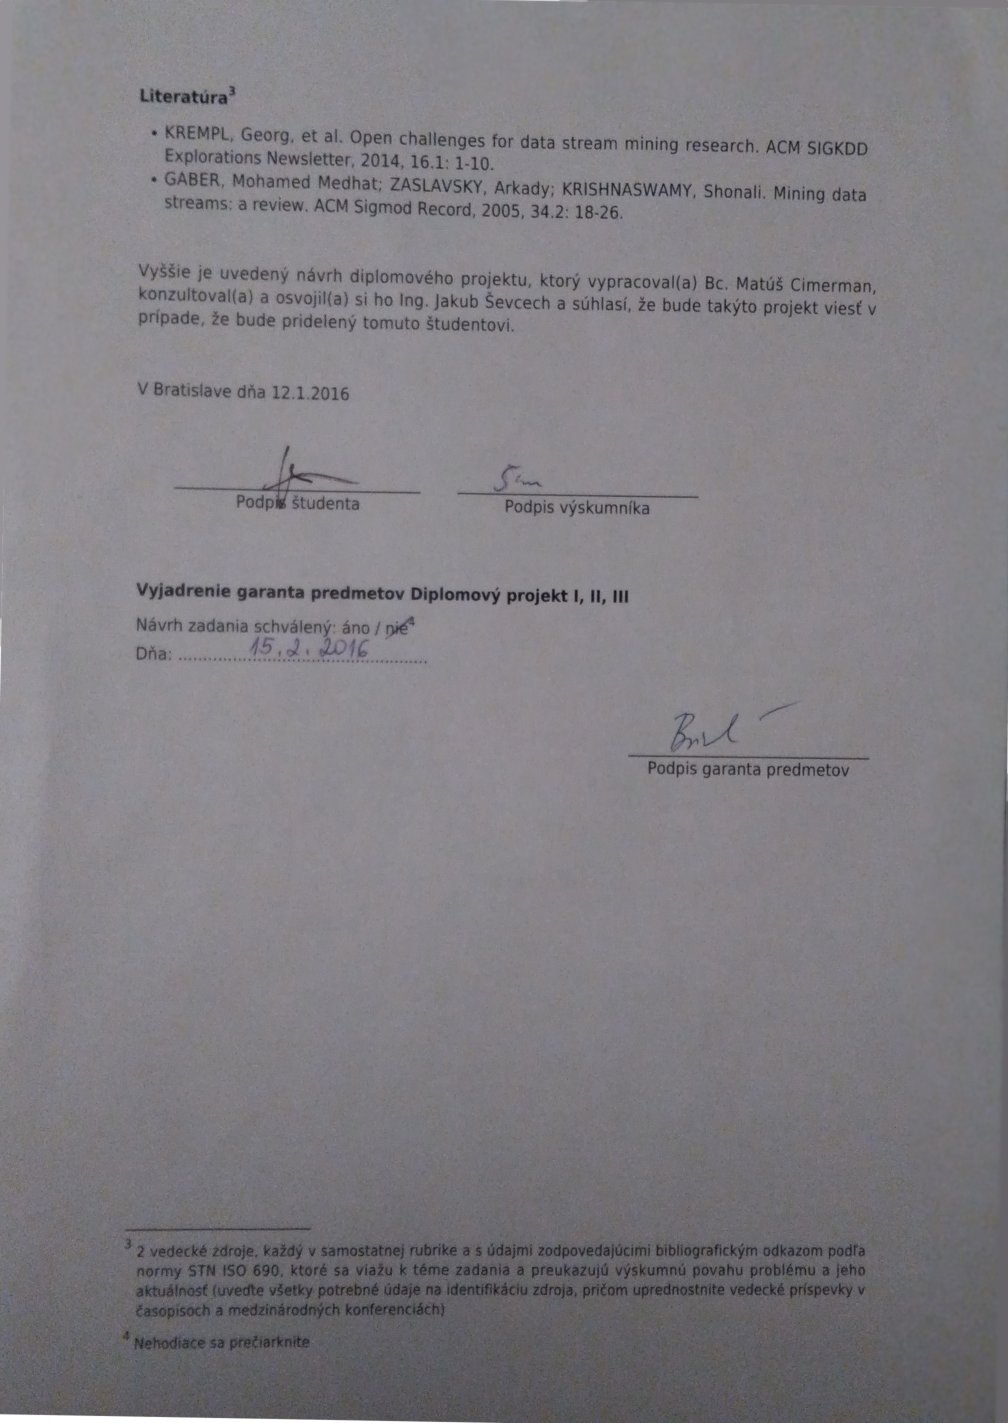
\includepdf[pages={1}]{navrh_2.pdf}

\includepdf[pages={1}]{zadanie.pdf}


%the abstract should include an english and a slovak version
\loadgeometry{myAbstract}
\chapter*{Anotácia\markboth{Abstrakt}{Abstrakt}}
%\addcontentsline{toc}{chapter}{\protect\numberline{}Abstrakt}
\label{abstrakt}
Slovenská technická univerzita v Bratislave\\
\MakeUppercase{Fakulta Informatiky a Informačných Technológií}

%\begin{tabular}{ p{15em} p{15em} }
\begin{tabular}{@{}p{15em} p{17.5em}}
Študijný program: & Informačné systémy\\
\\
Autor: & Bc. Matúš Cimerman\\
Diplomová práca: & Analýza prúdu prichádzajúcich udalostí použitím rôznych metód pre analýzu údajov\\
Vedúci diplomovej práce: & Ing. Jakub Ševcech, PhD.\\
máj 2017
\end{tabular}

\vspace{10mm}
%here (slovak version)
V súčasnosti pozorujeme narastajúci záujem a potrebu analyzovať dáta v čase ich vzniku. Použitie a interpretácia analytických metód v doméne spracovania údajov uvádza známy problém neviditeľnosti a porozumenia modelu. Jedným z nich je použitie tradičných dávkových metód pre prúdy dát, ku ktorým je potrebné hľadať iné alternatívy a druhou úlohou je interpretácia výsledného modelu a výsledkov. V oblasti prúdov dát je avšak fenoménu interpretácie modelu analytických metód venovaná len nepatrná pozornosť. Sústreďujeme sa najmä na problém interpretácie modelu za predpokladu, že doménový expert nedisponuje detailnými znalosťami o fungovaní modelu.
\par
Navrhujeme použitie rozhodovacieho stromu v úlohe klasifikácie prúdu dát, ktorý používa Hoeffdingovu mieru pre výber potrebného počtu pozorovaní pre každé rozhodnutie. Pre vysporiadanie sa so zmenami aplikujeme algoritmus ADWIN, ktorý adaptívne detekuje zmeny v prúde dát. Zameriavame sa na jednoduchosť vybranej metódy a interpretovateľnosť výsledkov. Pre doménových expertov je nevyhnutné, aby boli tieto požiadavky splnené, pretože nebudú potrebovať detailné znalosti z domén ako strojové učenie alebo štatistika. Avšak, znalosti dát, ich kontextu a významu jednotlivých atribútov sú nevyhnutné. Naše riešenie overujeme implementovaním vizualizácie a kvalitatívnym experimentom.


%=== ENGLISH VERSION===% 
\emptydoublepage
\chapter*{Annotation\markboth{Abstract}{Abstract}}
%\addcontentsline{toc}{chapter}{\protect\numberline{}Abstract}
\label{abstract}

Slovak University of Technology Bratislava\\
\MakeUppercase{FACULTY OF INFORMATICS AND INFORMATION TECHNOLOGIES}

%\begin{tabular}{ p{15em} p{15em} }
\begin{tabular}{@{}p{15em} p{17.5em}}
Degree course: & Information systems\\
\\
Author: & Bc. Matúš Cimerman\\
Master’s Thesis: & Stream analysis of incoming events using different data analysis methods\\
Supervisor: & Dr. Jakub Ševcech\\
2017, May
\end{tabular}

\vspace{10mm}

%here (english version)
Nowadays we are observing increasing demand in analyzing data as they arrive. Analysis and processing streaming data is complex task whereas it's important that implemented solution has low latency response time. Application and interpretation of analytical methods in data processing domain is well known issue. One of the problems is applicability traditional batch methods for streaming data. Model interpretation is separate challenge, however only tiny attention is paid to this phenomena. Therefore we particularly focus on model interpretation for domain expert. We assume domain expert does not have knowledge of machine learning algorithms.
\par
We propose application of decision tree in streaming data context. This decision tree is using Hoeffding bound to select best split attribute with a given confidence. To deal with concept drift we apply algorithm ADWIN as a black-box, which is suitable to adaptively detect changes in streaming data. The main focus and asset of this work is aimed to simplicity and interpretability results of given method. This is essential for domain experts since they do not need to have machine learning knowledge. However, understanding of data and its context is necessity. We implement visualization and evaluate it qualitatively with several domain experts.
\emptydoublepage
\loadgeometry{myText}

\emptydoublepage

%acknowledgements
\loadgeometry{myAbstract}

\chapter*{Poďakovanie\markboth{Poďakovanie}{Poďakovanie}}
%\addcontentsline{toc}{chapter}{\protect\numberline{}Poďakovanie}

\vfill
Na prvom mieste vyslovujem poďakovanie vedúcemu mojej diplomovej práce, Ing. Jakubovi Ševcechovi, PhD., za všetky jeho odborné rady, odovzdané skúsenosti a usmernenie pri tvorení práce. \\
Touto cestou taktiež vyslovujem poďakovanie všetkým výskumníkom zo skupiny PeWe, za prínosné diskusie a ich spätnú väzbu týkajúcu sa mojej práce. \\
V neposlednom rade ďakujem celej mojej rodine a priateľom.

\begin{flushright}
Matúš Cimerman
\end{flushright}


\loadgeometry{myText}


\emptydoublepage

%conventions applied in the thesis
%%!TEX root = ./main.tex
%
% This file is part of the i10 thesis template developed and used by the
% Media Computing Group at RWTH Aachen University.
% The current version of this template can be obtained at
% <http://www.media.informatik.rwth-aachen.de/karrer.html>.

\chapter*{Conventions\markboth{Conventions}{Conventions}}
\addcontentsline{toc}{chapter}{\protect\numberline{}Conventions}

Throughout this thesis we use the following conventions.



\bigskip

\emph{Text conventions}

Definitions of technical terms or short excursus are set off in coloured boxes.

\myDefBox{Excursus}
{Excursus are detailed discussions of a particular point in a book, usually in an appendix, or digressions in a written text.}

\medskip

Source code and implementation symbols are written in typewriter-style text.

\texttt{myClass}

\medskip

The whole thesis is written in Canadian English.

\medskip

Download links are set off in coloured boxes.

\myDownloadURL{File: myFile}{file_number.file}{file\myUnderscore number.file}

%\pagebreak

%\emph{Formula conventions}




%\emptydoublepage

\renewcommand{\contentsname}{Obsah}
\singlespacing
\tableofcontents

\emptydoublepage
\onehalfspacing
%\doublespacing
%
%\listoffigures
%\emptydoublepage
%
%\listoftables
%\emptydoublepage

\newtheorem{definition}{Definícia}[section]
\newtheorem{hypothesis}{Hypotéza}[section]


%--------------------------------------------------------------
% hlavny obsah
%--------------------------------------------------------------
\mainmatter

%!TEX root = ./main.tex

\chapter{Úvod}
%\label{introduction}
V súčasnosti pozorujeme zvýšený záujem o oblasť analýzy a dolovania dát. Vhodné použitie a výber metód pre analýzu dát prináša hodnotné výstupy a náhľady pre doménového experta, ktoré môžu byť použité pre strategické rozhodnutia v podnikoch. Najčastejší postup je aplikovanie metód ako lieviková analýza alebo rozhodovacie stromy nad statickou kolekciou dát. Príkladom lievikovej analýzy môže byť snaha zistiť v ktorej časti nákupného procesu na internetovom obchode odchádza najväčšie percento zákazníkov. V prípade rozhodovacích stromov nás môže zaujímať klasifikácia zákazníka, ktorá ukáže či zákazník opustí internetový obchod. Na základe týchto výsledkov je možné dodatočne predložiť zákazníkovi jedinečnú ponuku a vďaka tomu zvýšiť zisk spoločnosti. Tento prístup má niekoľko problémov, medzi ktoré patrí predovšetkým: všetky trénovacie dáta musia byť uložené v pamäti alebo na disku; spracovanie a výpočtová náročnosť; vysporiadanie sa s trendami a zmenami v dátach. Nutnosť najskôr zozbierať a následne uložiť rýchlovznikajúce dáta predstavuje rovnako veľký problém ako ich samotné následné spracovanie.
\par
Pod pojmom spracovanie dát v reálnom čase rozumieme spracovanie v takmer reálnom čase, tzv. jemné (angl. soft) spracovanie v reálnom čase. Jemné spracovanie v reálnom čase v porovnaní s mohutným (angl. hard) spracovaním nezaručuje spracovanie vzorky v stanovenom čase, pričom niektoré vzorky sa môžu omeškať alebo úplne vynechať \citep{stankovic1988real}. Presné limity ohraničujúce spracovanie v reálnom čase závisia od konkrétného problému. Niekedy to môže predstavovat rádovo stotiny sekundy inokedy môže ísť rádovo o sekundy. V tejto práci budeme pracovať s pojmom spracovanie v reálnom čase chápajúc ho ako jemné spracovanie v reálnom čase.
\par
Pri dolovaní v prúde dát čelíme niekoľkým výzvam: objem,  rýchlosť (frekvencia) a rozmanitosť. Veľký objem dát, ktoré vznikajú veľmi rýchlo, je potrebné spracovať v ohraničenom časovom intervale, často v reálnom čase. Keďže sa objem dát neustále zväčšuje, potenciálne narastá až donekonečna. Identifikovali sme niekoľko najviac zasiahnutých oblastí, ktoré sú zdrojmi týchto dát: počítačové siete, sociálne siete, webové stránky (sledovanie správania používateľa na stránke) a Internet Vecí (angl. Internet of Things). Na informácie generované z takýchto zdrojov sa často pozeráme ako na neohraničené a potenciálne nekonečné prúdy údajov.
\par
Spracovanie, analýza a dolovanie v týchto prúdoch je komplexná úloha. Pre aplikácie je kritické spracovať údaje s nízkou odozvou, pretože riešenie musí byť presné, škálovateľné a odolné voči chybám. Nakoľko sú prúdy neohraničené vo veľkosti a potenciálne nekonečné, môžeme spracovať len ohraničený interval prúdu. V takomto prípade je potrebné dáta spracovať v čase ich vzniku. Tradičné metódy a princípy pre spracovanie statickej kolekcie údajov nie sú postačujúce na takéto prípady \citep{krempl2014open, han2011data}. Za tradičné metódy považujeme také, ktoré potrebujú najprv všetky dáta zozbierať, a potom nad vytvorenou dátovou kolekciou aplikujú metódy dolovania dát. Programovacie paradigmy ako MapReduce, na ktorých sú založené programovacie rámce ako napríklad Apache Spark \footnote{http://spark.apache.org/}, umožnili distribuované spracovanie veľkých objemov dát v akceptovateľnom čase. Problémom stále ostáva neustály nárast objemu dát, ktorý nie je ohraničený, a spracovanie v reálnom čase. Adaptácia na zmeny tiež často nie je zohľadená v týchto metódach. Zmeny môžu byť rôzneho charakteru, napríklad náhle alebo postupné, či opakované.
\par
Cieľom našej práce je analýza súčasných metód pre spracovanie a analýzu prúdu údajov a ich následné aplikovanie vybranej metódy v zvolenej doméne. Pre metódu analýzy prúdu údajov sme si zvolili metódu rozhodovacích stromov v úlohe klasifikácie. Kladieme dôraz na spracovanie v reálnom čase, ktoré je najzákladnejšie pri spracovaní prúdov dát. Veľkú pozornosť pritom mierime na schopnosť adaptácie metódy na zmeny v dátach. Výsledný model zobrazujeme vizualizáciou s cieľom uľahčiť pochopenie a interpretáciu výsledkov. Keďže neexistujú práce, ktoré sa priamo venujú a vyhodnocujú vizualizácie modelov nad prúdmi dát, rozhodli sme sa aplikovať vizualizáciu pre algoritmus rozhodovacích stromov učiacich sa v reálnom čase. Súčasťou práce je tiež návrh architektúry a prototyp implementácie potrebnej pre aplikovanie spomenutej metódy spolu s vizualizáciou.
\par
V druhej kapitole práce sa venujeme detailnej analýze rôznych analytických úloh nad prúdmi dát. Spolu s každou úlohou analyzujeme tiež metódy a algoritmy, ktoré sú vhodné pre jej riešenie. Jednou z týchto úloh je napríklad klasifikácia, ktorej venujeme najväčšiu pozornosť. Tretia kapitola hovorí o probléme interpretácie a vysvetlení výsledkov používateľovi. V štvrtej kapitole analyzujeme existujúce analytické a vizualizačné nástroje. V piatej a šiestej kapitole navrhujeme a popisujeme implementáciu metódy rozhodovacích stromov, potrebnej architektúry a vizualizácie. V poslednej kapitole vyhodnocujeme kvantitatívne a kvalitatívne implementovanú metódu.











\emptydoublepage
%\chapter{Otvorené problémy pri analýze prúdu údajov}
\label{Otvorené problémy pri analýze prúdu údajov}
Dolovanie a objavovanie znalostí, alebo tiež analýza a spracovanie prúdu dát čelí trom hlavným výzvam: \textit{objem}, \textit{rýchlosť} a \textit{nestálosť} dát \citep{krempl2014open}. 

\section{Použitie tradičných metód dolovania dát a strojového učenia}

\section{Evaluácia modelov a algoritmov}

\section{Vizualizácia výsledkov používateľovi}

\section{Technické výzvy}

%\emptydoublepage
\include{methods}
\emptydoublepage
\chapter{Analytické úlohy nad prúdom dát}
\label{Analytické úlohy v prúde dát}
Spracovanie, analýza a dolovanie dát predstavuje vo všeobecnosti výzvu. Zvláštnu pozornosť si tieto úlohy vyžadujú pri spracovaní, analýze a dolovaní z prúdu udalostí. Prúd udalostí je často nazývaný \textit{prúd dát} alebo \textit{údajov}, či len skrátene \textit{prúd}. V tomto texte budeme pre jednoduchosť používať najmä termín \textit{prúd} a \textit{prúd dát}. Avšak v literatúre sa môžu vyskytnúť aj termíny ako \textit{prúd udalostí}, \textit{sekvencia udalostí, či elementov}, pričom všetky termíny majú v tomto texte \textit{rovnaký} význam. 
\par
\begin{definition}{Prúd je potenciálne nekonečná sekvencia elementov \citep{tran2014change}.}
\begin{align*}
	S = \{(X_1,T_1), ..., (X_j,T_j), ...\}
\end{align*}
Kde každý element je pár $(X_j,T_j)$ kde $X_j$ je d-dimenzionálny vektor $X_j = (x_1, x_2, ..., x_d)$ prichádzajúci v čase $T_j$. $T_j$ je často nazývaný aj časová pečiatka, existujú dva typy časovej pečiatky: explicitná je generovaná keď dáta dorazia, implicitná je priradená vektoru v čase ich vzniku.
\end{definition}

% Vseobecny popis toho preco je potrebne prudove spracovanie dat
Takmer každé odvetvie, napríklad telekomunikačné siete alebo predajné reťazce, je dnes zdrojom masívnych objemov dát. Vzhľadom na ich veľký objem analytyci a doménoví experti často strácajú možnosť dolovať v celej sade dát. Zvykom preto býva použiť distribuované paradigmy a umožniť tak dolovanie v celej kolekcii dát, čo je ale náročné na vývoj a čas spracovania. Stáva sa preto častým zvykom, že sa vyberie reprezentatívna vzorka, ktorej spracovanie predstavuje menšiu časovú a pamäťovú výzvu. Pri pamäťovej a výpočtovej náročnosti hovoríme o hardvérových limitoch počítača, pričom ak hovoríme o časovej náročnosti hovoríme o limitovanom čase doménového experta (čakanie na výsledok analýzy) \citep{hulten2001mining}. Predpokladajme, že bude pre doménoveho experta vysokým prínosom možnosť vykonávať analýzy nad prúdom v reálnom čase. Výstupy z takejto analýzy sú na rôznej granularite a úrovni, pričom môžu byť neskôr použité na ďalšie spracovanie alebo na priame prezentovanie výsledkov.
\par
Problém analýzy dát bol veľmi dobre a podrobne študovaný pri spracovaní statickej kolekcie údajov. Pri tomto prístupe sú všetky dáta v pamäti počítača. Vybraný algoritmus potom môže pomerne jednoducho prečítať celú množinu niekoľkokrát s cieľom zvýšenia presnosti a kvality výsledného modelu. Tento prístup nie je aplikovateľný v doméne prúdov dát z nasledujúcich dôvodov:
\begin{itemize}
	\item \textit{Prúd dát je potenciálne nekonečná sekvencia udalostí}, ktoré môžu byť správne alebo chybne usporiadané v závislosti od spoľahlivosti zdroja dát. Hlavný problém tu predstavuje to, že prúd je nekonečná sekvencia udalostí. Závažnosť problému usporiadania daných udalostí, či vozriek závisí od konkrétnej úlohy analýzy prúdu dát.
	\item \textit{Obmedzená pamäť} značí, že nie je možné všetky dáta zbierať a ukladať do pamäti. Toto obmedzenie vyplýva z prvej vlastnosti prúdov dát.
	\item \textit{Model pre klasifikáciu prúdov musí byť ihneď pripravený k použitiu.} Znamená to, že hneď po tom ako sú spracované prvé dáta z prúdu je model pripravený na použitie, napríklad klasifikovať iný prúd dát.
	\item \textit{Prúdy dát takmer vždy v sebe nesú zmeny} (angl. concept drift), na ktoré sa musí vedieť klasifikátor adaptovať. Vlasnosť klasifikačných modelov vysporiadať sa so zmenami považujeme za rozhodujúcu pri hodnotení ich kvality a použiteľnosti v praxi. Preto sa aj nami navrhovaná metóda sústreďuje na vytvorenie metódy schopnej adaptácie na zmeny a ich adekvátne interpretovanie používateľovi. Zmeny v dátach môžu byť náhle, postupné ale môžu predstavovať aj očakávané sezónne vplyvy (napr. obdobie Vianoc z pohľadu počtu nákupov internetového obchodu).
\end{itemize}

% Vyskumne vyzvy v prudoch dat vseobecne
Analýza a spracovanie prúdov dát pridáva viaceré otvorené výzvy a možnosti pre výskum \citep{krempl2014open}:
\begin{itemize}
	\item \textit{Ochrana súkromia a dôvernosti} pri analýze a dolovaní v prúde dát. Hlavným cieľom je vyvinúť metódy a techniky odhaľujúce informácie a vzory, ktoré by znížili dôveryhodnosť a povinnosti ochrania súkromia. Dve hlavné výzvy pri analýze a dolovaní v prúdoch dát sú: \textit{vysporiadanie sa s neúplnými dátami} a \textit{uchovanie zmien (angl. concept drift) v prúde dát}. Neúplné dáta môžu začať prichádzať zámerne, napríklad po útoku na počítačovú sieť. Zmeny v distribúcií dát môžu opäť podobne nastať po útoku na sieť. Pre vysporiadanie sa s podobnými javmi je často do prúdu dát zámerne pridávaný šum, čo je do istej miery v rozpore s problémom predspracovania dát.
	\item \textit{Predspracovanie dát} je dôležitou súčasťou každej reálnej aplikácie, najmä tých pre analýzu dát. Zatiaľ čo pri tradičnej analýze dát je predspracovanie vykonané, zvyčajne doménovým expertom, ktorý rozumie dátam. Pri prúde dát toto nie je prijateľné, pretože dáta nepretržite prichádzajú. Okrem niekoľkých štúdií \citep{zliobaite2014adaptive, anagnostopoulos2008deciding} tejto problematike nebola venovaná toľká pozornosť ako pri tradičnom spracovaní a analýze dát. Hlavné výzvy, ktorým treba čeliť pri predspracovaní prúdu dát sú: \textit{šum v dátach}, \textit{hodnoty mimo väčšiny (angl. outliers)} a \textit{adaptívny výber vzorky}.
	\item \textit{Načasovanie a dostupnosť informácie} je dôležité pre väčšinu algoritmov, ktoré predpokladajú, že prijatá informácia je kompletná, ihneď dostupná, prijatá pasívne a zadarmo. Viaceré výzvy spojené s načasovaním a dostupnosťou informácie nie sú formulované a nepreskúmané: \textit{spracovanie nekompletných dát}, \textit{vysporiadanie sa so skreslenou (angl. skewed) distribúciou dát} a \textit{spracovanie oneskorených dát}.
	\item \textit{Dolovanie entít a udalostí}, kde entity sú vytvorené z viacerých inštancií prúdu dát a vytvárajú tak štruktúrované informácie (napr. agregácie). Tieto entity môžu byť niekedy spojené s výskytom udalostí. Príkladom takejto entity, či udalosti môže byť zhluk správ o zemestrasení na sociálnej sieti Twitter. 
	\item \textit{Evaluácia algoritmov pre prúdy dát} predstavuje úplne novú výzvu v porovnaní s tradičnými metódami. Pri evaluácií v prúde dát sa musíme vysporiadať s problémami ako napr.: \textit{zmeny (angl. concept drift)}, \textit{limitovaný čas pre spracovanie vzorky}, \textit{vyvíjajúce sa skreslenie tried dát}, či \textit{oneskorenie overenia}. Tejto problematike sa v poslednej dobe venuje vyššia pozornosť, ako napríklad pre evaluáciu klasifikátorov nad prúdmi dát \citep{bifet2015efficient}.
\end{itemize}

% Model prudu dat
\paragraph{Model prúdu dát} môže byť jeden z nasledujúcich: \textit{model časových radov}, \textit{pokladničný} model a model \textit{turniketu}. Podľa modelu prúdu dát existujú príslušné algoritmy, ktoré boli vytvorené pre daný model \citep{tran2014change}. Majme prúd dát $a_1, a_2, ...$, ktorý prichádza sekvenčne za sebou a popisuje sledovaný signál $A$. 
V modeli časových radov každá vzorka $a_i$ sa rovná $A[i]$, pričom vzorky prichádzajú vo vzostupnom poradí. Tento model je vhodný pre prúdy dát, ktoré nesú v sebe časovú postupnosť alebo je ich poradie určované časovou pečiatkou \citep{muthukrishnan2005data}.
Pri pokladničnom modeli môžme považovať množinu $U = {1, 2, ..., n}$ za element z prúdu dát, kde $n$ je počet vzoriek z prúdu. Sekvencia $2, 1, 2, 5$ môže byť považovaná za príklad pokladničného modelu. Tento model je často používaný v praxi, napríklad v prípadoch kde následnosť IP adries pristupuje na Web server \citep{ikonomovska2013algorithmic, muthukrishnan2005data}.
Model turniketu je veľmi podobný pokladničnému modelu. Rozdiel je v tom, že vzorka môže predstavovať aj zápornú hodnotu. Ide o analógiu z reálneho sveta kedy niektorí ľudia vchádzajú a ďalší zároveň vychádzajú turniketom, vtedy sa počet ľudí mení (napr. na zjazdovke) \citep{ikonomovska2013algorithmic, muthukrishnan2005data}. Špeciálny striktný prípad turniketu, ak celková hodnota modelu je $A \geq 0$.

% Predspracovanie prudu dat
\paragraph{Predspracovanie prúdu} je neodmysliteľným krokom v aplikáciach reálneho sveta a často časovo najnáročnejšou úlohou pre každého analytika. Nakoľko dáta prichádzajú z nehomogénneho sveta, môžu byť zašumené, nekompletné, duplicitné alebo často obsahujú hodnoty značne líšiace sa od ostatných. Predspracovanie prúdu údajov je potrebné čo najviac automatizovať. Existuje niekoľko známych metód a techník, ktoré sú používané pri predspracovaní a tiež pri redukcii dimenzionality prúdov dát \citep{krempl2014open, nguyen2015survey}:
\begin{itemize}
	\item \textit{Vzorkovanie}, napríklad použitím symbolickej reprezentácie časových radov v prúde dát. Takáto reprezentácia nám umožňuje redukciu veľkosti prenášaných dát. Daná technika pozostáva z dvoch hlavných krokov, aproximácia po častiach a následná transformácia výsledku do diskrétnych veličín \citep{sevcech2015symbolic}. 
	\item \textit{Zahadzovanie potenciálne nepotrebných vzoriek} sa uplatňuje vtedy, keď je spracujúci proces príliš zaťažený. Tu môže nastať problém, ak práve zahodená vzorka bola niečím dôležitá (napr. zmena v dátach).
	\item \textit{Agregácia údajov} môže značne znížiť objem dát, ale môže spôsobiť problém pri potrebe náhľadu do minulosti na pôvodné dáta, z ktorých vznikla. Jednou z metód, ktorá sa používa na výpočet dopytovaných agregácií nad prúdom dát je vytváranie malých sumárov z $n$ vzoriek prúdu. Tieto náhodne veľké sumáre sú použité pre výpočet agregácie \cite{dobra2002processing}.
	\item \textit{Aproximačné algoritmy} a ich použitie má za následok podstatné zrýchlenie spracovania a analýzy prúdov za predpokladu istej chybovosti. Chybovosť je zväčsa ohraničená.
	\item \textit{Posuvné okno} je prístup, ktorý vznikol s potrebou analýzy definovaného časového intervalu z prúdiacich údajov. Výstup je teda závislý na zvolenej veľkosti okna. Problém pri tomto prístupe je práve správne nastavenie veľkosti okna tak, aby sme vedeli zohľadniť zmeny v prúde dát.
\end{itemize}

\paragraph{Ohraničenia} algoritmov pre dolovanie z prúdov dát (angl. data stream mining) musia spĺňať nasledujúce podmienky \citep{babcock2002models, nguyen2015survey, wadewale2015survey}:
\begin{itemize}
	\item \textit{Jeden priechod cez dáta} (angl. single-pass) v dôsledku kontinuálneho spracovania vzoriek z nekonečného prúdu dát v čase ich vzniku, čo je v kontraste s tradičnými metódami, ktoré si udržiavajú všetky dáta v pamäti alebo na disku.
	\item \textit{Odpoveď v reálnom čase}  (angl. anytime real-time response) v zmysle, že vytvorený model je pripravený kedykoľvek predikovať triedy nových vzoriek.
	\item K dispozícii máme len \textit{ohraničenú pamäť}. Toto obmedzenie súvisí s povahou prúdov dát a to, že prúdy predstavujú potenciálne nekonečné zdroje dát.
	\item \textit{Detekcia zmien} (angl. concept-drift detection) je nevyhnutná v situácii, keď sa v dátach objavia nové vzory meniace sa v čase.
\end{itemize}

% Dolovanie a extrakcia informacii
\paragraph{Spracovanie, dolovanie a analýza dát} zo statických kolekcií dát bola študovaná niekoľko dekád. Zvýšenú pozornosť začala odborná verejnosť venovať pri aplikovaní týchto úloh na prúdy dát. Niektorým z týchto úloh sa venujeme podrobne v nasledujúcich podkapitolách:
\begin{itemize}
	\item \textit{Zhlukovanie} je úloha učenia bez učiteľa. Existuje niekoľko výskumov, ktoré sa venovali špeciálne klastrovaniu implementovaním napríklad k-mediánu a inkrementálnych algoritmov.
	\item \textit{Klasifikácia} predstavuje úlohu učenia s učiteľom, znamená to, že na vstupe očakávame označkovaný prúd dát. Táto úloha je dlho skúmaná s použitím mnohých metód, napríklad neurónových sietí, či rozhodovacích stromov.
	\item \textit{Hľadanie frekventovaných vzorov} za pomoci posuvných okien a inkrementálnych algoritmov sa využíva na detekciu vzorov v prúde. Príkladom tejto úlohy može byť napríklad hľadanie trendov v prúde dát alebo analýza nákupného košíka v doméne internetového obchodu.
\end{itemize}

% Evaluacia
\paragraph{Evaluácia} a vyhodnotenie modelov vytvorených nad prúdmi dát je základná a dôležitá úloha pre meranie kvality modelu, čo sebou prináša výzvy, pretože prúdy dát sú potenciálne nekonečné. Evaluáciu modelov je potrebné vykonávať online, pretože dáta môžu byť napríklad nerovnomerne rozdelené v prúde dát, čo predstavuje problém. Potom, tradičné techniky evaluácie známe z dávkových algoritmov pre analýzu dát nie sú použiteľné pre evaluáciu prúdov dát. \citet{bifet2015efficient} hovoria o troch hlavných mylných prístupoch k evaluácii prúdu dát:
\begin{itemize}
	\item \textit{McNemarov test} a jeho použitie na štatistické rozlíšenie kvality dvoch klasifikátorov. Aj napriek štatisticky signifikantnému rozdielu medzi klasifikátormi tento test nie je vhodný pre prúdy dát, pretože aj keď je model vytvorený rovnakým algoritmom, väčšina algoritmov je inicializovaná alebo používa nejakú náhodnú zložku. To môže viesť k zavádzajúcim výsledkom pri použití tohto testu.
	\item \textit{Rozdeľovanie množiny dát} do trénovacej a testovacej množiny vedie k nemožnosti rozoznať rýchlosť učenia rôznych klasifikátorov. Je to z dôvodu, že v dátach sa môžu objavovať napríklad zmeny, ktoré budu skreslené rozdeľovaním alebo vzorkovaním dát.
	\item \textit{Väčšina tried v posuvnom okne} môže spôsobiť pozitívne \textit{k štatistiky} a tiež pozitívne výsledky harmonického priemeru pre niektoré periódy prúdu dát.
\end{itemize}

\citet{bifet2015efficient} odporúčajú použitie nasledujúcej metódy pre evaluáciu v kontexte prúdov dát: \textit{Najprv testuj-potom-trénuj} (angl. Test-Then-Train alebo tiež Prequential) spočíva v myšlienke, že každá vzorka z prúdu dát je použitá najprv na testovanie a potom na trénovanie modelu. Keďže modely vytvorené nad prúdmi dát by mali byť schopné poskytnúť predikcie okamžite a v reálnom čase, tento prístup by nemal výrazne ovplyvniť výkon metódy. Obmenou tohto prístupu môže byť evaluácia na nejakom posuvnom okne.


%%%%%%%%%%%%%%%%%%%%%%%%%%%%%%%%%%%%%%%%%%%%%%%%%
%         Dopytovanie sa v prúdoch dát          %
%%%%%%%%%%%%%%%%%%%%%%%%%%%%%%%%%%%%%%%%%%%%%%%%%
\section{Dopyty nad prúdom dát}
Vyhodnocovaniu dopytov nad statickou kolekciou dát bola v minulosti venovaná značná pozornosť, ak však hovoríme o prúdoch dát dopyty musia byt vyhodnocované kontinuálne \citep{babu2001continuous, babcock2002models}. Vzniká teda nová paradigma pre interakciu s dynamicky sa meniacimi dátami, ktorú nazývame kontinuálne dopyty (angl. continious queries) \citep{babu2001continuous}. Výsledky kontinuálnych dopytov sú produkované dynamicky v čase vzniku nových dát. Príkladom použitia takýchto dopytov je napríklad sledovanie vývoja akcií burzy. Problém môže nastať pri jednorázových dopytoch obsahujúce agregačné funkcie. Pri tradičnom spracovaní dát uložených ako statická kolekcia je dopyt vykonaný nad celou kolekciou. V prípade kontinuálneho dopytu je problém získať predchádzajúce dáta za predpokladu, že dáta niesú ukladané. Potom môžu nastať dve situácie:
\begin{enumerate}
	\item agregačná funkcia je prepočítaná zo sumárov získavaných priebežne z prúdu dát.
	\item agregačná funkcia je počítaná od momentu zadania dopytu.
\end{enumerate}
Kontinuálne dopytovanie do prúdu dát nesie so sebou nieľko výziev \citep{babcock2002models}:
\begin{itemize}
	\item \textit{Limitované pamäťové prostriedky} na algoritmy spracujúce dopyty, pretože prúd dát predstavuje potenciálne nekonečný prúd udalostí.
	\item \textit{Približné odpovede na dopyty} sú niekedy postačujúce za predpokladu, že odpoveď je dostatočne rýchla a používateľ je oboznámený v akej presnosti mu bola odpoveď poskytnutá. Techniky pre redukciu dimenzionality a objemu dát zahŕňajú napríklad: histogramy, náhodné vzorkovanie, symbolické vzorkovanie a pod.
	\item \textit{Dopytovací jazyk} by mal byť podobný jazyku SQL. Jazyk SQL je známy široko používaný deklaratívny jazyk so zavedeným štandardom, ktorý poskytuje flexibilitu a optimálne vykonanie dopytu.
\end{itemize}
Výskumné práce sa tiež venovali adaptívnym kontinuálnym dopytom nad prúdmi dát. Bolo ukázané, že takýto prístup môže mať značný prínos v oblasti výkonnosti systému vďaka jeho schopnosti adaptácie na zmeny v prúde dát. Tieto vlastnosti sú dosiahnuté aplikovaním zoskupovania indexov filtrov na priebežný výber predikátov \citep{madden2002continuously}. 
\par
Ďalší priestor na zlepšenie výkonnosti kontinuálnych dopytov nad prúdmi dát predstavujú adaptívne filtre. Pri dopytovaní sa takmer vždy vykonáva filtrovanie dát v nejakej podobe. Tento krok filtrovania je obvykle implementovaný v systéme na spracovanie dopytov. Pre zvýšenie výkonnosti dopytov je preto možné tieto filtre presunúť priamo do zdrojov dát. Ukázalo sa, že takýto prístup môže mať pozitívny dopad na výkonnosť \citep{olston2003adaptive}. Tento prístup prinesie najmä redukciu prenášaných dát výmenou za ich neúplnosť alebo nepresnosť. Výzvou tejto techniky je, že je aplikovateľná len v kontrolovanom prostredí, do ktorého všetkých súčastí vieme zasahovať. Príkladom môže byť organizácia CERN\footnote{Európska organizácia pre jadrový výskum}, ktorej jeden z hlavných experimentov ATLAS produkuje Petabajty dát počas jedného experimentu. Takéto množstvo dát by nebolo možné ukladať a následne analyzovať, preto sú aplikované filtre v každom zdroji dát (napr. rôzne fyzikálne senzory).



%%%%%%%%%%%%%%%%%%%%%%%%%%%%%%%%%%%%%%%%%%%%%%%%%
%               Detekcia zmien                  %
%%%%%%%%%%%%%%%%%%%%%%%%%%%%%%%%%%%%%%%%%%%%%%%%%
\section{Detekcia zmien}
Detekcia zmien (angl. concept drift) zohráva v dnešnom rýchlo sa meniacom svete dôležitú úlohu. Zmeny nastávajú veľmi rýchlo a nečakane. Preto stúpa potreba detekcie zmeny a následná správna reakcia, ktorá vyplynie z detekovanej zmeny. Na to, aby sme boli schopní na tieto zmeny adekvátne reagovať, je potrebné dáta spracovávať tak, ako vznikajú a pozerať sa na ne ako na prúd udalostí. Tradičné metódy pre paralelné spracovanie uvažujú len statickú kolekciu dát \citep{tran2014change}. Existuje niekoľko typov zmien, ktoré môžu nastať v prúde dát \citep{wadewale2015survey}: \textit{náhla} (angl. sudden), \textit{inkrementálna}, \textit{graduálna}, \textit{opakujúca}, \textit{impulzívna} a \textit{šum}. Spomenuté zmeny sú zobrazené na obrázku \ref{fig:types-of-concept}.
\myFigure{images/types-of-drift}{Typy zmien (angl. concept drift) \citep{wadewale2015survey}.}{test-dia}{0.5}{h!}\label{fig:types-of-concept}
Detekcia zmeny predstavuje proces identifikácie zmeny aktuálneho stavu modelu voči predchádzajúcemu. Na tento model sa pozeráme v rôznom čase. Dôležitý rozdiel medzi zmenou a rozdielom je, že zmena hovorí o prechode modelu do iného stavu, zatiaľ čo rozdiel znamená nepodobnosť v atribútoch dvoch modelov. V kontexte prúdu je detekcia zmien proces segmentácie do rôznych segmentov a identifikácia miest s meniacou sa dynamikou\citep{ross2009online}. Metóda pre detekciu zmien musí riešiť nasledujúce úlohy \citep{tran2014change}: 
\begin{itemize}
	\item \textit{detekcia zmeny} znamená správnu identifikáciu zmeny,
	\item \textit{lokalizácia zmeny} hovorí o identifikovaní momentu kedy, zmena nastala.
\end{itemize}
 Týmto úlohám je potrebné venovať dostatočnú pozornosť, pretože zmeny môžu byť falošné alebo dočasné, čo so sebou prináša problém lokalizácie danej zmeny. Ďalší termín, ktorý je potrebné zadefinovať je detekovaná zmena (angl. concept drift). Detekcia concept drift-u sa sústreďuje na označkované dáta, zatiaľ čo detekcia zmeny pracuje aj s neoznačkovanými dátami. Označkované dáta pre detekciu concept drift-u sú dôležité, pretože nás zaujíma skutočný význam a hodnota pozorovaní. Naopak, pri detekcii zmien niekedy môže byť postačujúce sledovať zmenu v distribúcií dát alebo početnosti. V praxi sa ale ukázalo, že aj detektory, ktoré sú do istej miery založené na sledovaní zmeny distribúcie dát dokážu úspešne detekovať concept-drift.
 \par
Metódy pre detekovanie zmien môžme klasifikovať do nasledujúcich prístupov \citep{liu2010mining}: \textit{metódy založené na stave}, \textit{metódy sledujúce trend} a \textit{prahové metódy}. Algoritmus pre detekciu zmien by mal spĺňať aspoň nasledovné požiadavky: \textit{presnosť}, \textit{rýchlosť} a \textit{odpoveď v reálnom čase}. Algoritmus by tiež mal detekovať čo najmenej chybných zmien a čo najviac správnych presných miest zmeny. Algoritmy by mali byť prispôsobené reálnemu prostrediu a spracovaniu prúdov vysokých objemov a rýchlostí. Na obrázku \ref{fig:zmeny-vseobecny-dia} je zobrazený všeobecný diagram pre detekciu zmeny v prúde udalostí.

\myFigure{images/2_zmeny_vseobecny-diagram}{Všeobecný diagram zobrazujúci detekciu zmeny v prúde udalostí \citep{tran2014change}. Komponent slúžiaci na dolovanie v prúde dát implementuje detektory zmien. Podľa výstupov týchto detektorov sa výsledný model adaptuje a zohľadňuje zmeny na vstupe.}{test-dia}{0.5}{h!}\label{fig:zmeny-vseobecny-dia}

% Techniky a metody pre detekciu zmeny v prudoch
Pre detekciu zmeny v prúdoch dát bolo vyvinutých niekoľko techník a metód. Niektoré z nich nižšie podrobnejšie popisujeme.

% Charakteristika dat
 Jeden z druhov metódy pre detekciu zmien zohľadňuje \textit{charakteristiku dát}. Najčastejšie môžme prúdy klasifikovať do kategorických (n-tice, množiny) alebo numerických prúdov. Ak hovoríme o kategorických prúdoch, dáta obsiahnuté v prúde majú kategorický charakter, príkladom sú rôzni výrobcovia áut: $x \in \{Volvo, Toyota\}$. Pri numerických prúdoch dáta predstavujú numerické hodnoty $x \in {\rm I\!R}$. Pre každý takýto prúd boli vyvinuté príslušné algoritmy. Problém nastáva pri aplikáciach s dátami reálneho sveta, kedy prúdy často obsahujú numerické aj kategorické dáta. V takýchto situáciach má zmysel dáta rozdeliť do rovnomenných skupín obsahujúce dáta rovnakého typu. Na tieto skupiny sú následne použité príslušné algoritmy. Prúdy dát sa ďalej môžu klasifikovať do označkovaných a neoznačkovaných prúdov. Neoznačkované prúdy obsahujú dáta nezaradené do žiadnej triedy. Naopak označkované prúdy nesú v sebe informáciu o tom, do ktorej triedy patrí vybraný element. Príkladom opísaného prúdu môže byť prúd nákupov internetového obchodu. Rôzny charakter prúdu predstavuje rôzne zmeny a prístup na ich riešenie pri detekcii zmien v prúde \citep{tran2014change}.

% Kompletnost statistickej informacie
\textit{Metóda pre detekciu zmeny} sa označuje skratkou DDM z anglického Drift Detection Method. Je to metóda zaoberajúca sa detekciou zmeny modelu. Majme prúd dát $(x_i,y_i)$ kde $x_i$ predstavuje atribúty a $y_i$ skutočnú triedu vzorky. Model sa potom snaží predikovať skutočnú triedu $y_{i+1}$ novej vzorky. Gama a spol. založili DDM na fakte, že každá iterácia klasifikátora predikuje triedu vzorky. Klasifikátor je binárny, takže trieda môže byť len $pravda$ alebo $nepravda$. Potom pre množinu vzoriek chyba predstavuje náhodnú premennú z Bernoulliho pokusov (angl. Bernoulli trials). Vďaka tomu môžme chybu modelovať s bínomickým rozdelením. Nech $p$ je pravdepodobnosť zlej predikcie a $s_i$ je štandardná odchýlka vypočítaná nasledovne:
\begin{align*}
s_i = \sqrt{ \frac{p_i(1-p_i)} {i} }
\end{align*}
Pre každú vzorku z prúdu sú udržiavané dve premenné, $p_{min}$ a $s_{min}$. Ich hodnoty sú použité na výpočet varovnej hodnoty, ktorá slúži na definovanie optimálnej veľkosti kontextového okna. Kontextové okno si udržiava staré vzorky obsahujúce nový kontext, resp. zmenu, či posun pojmu a minimálny počet elementov zo starého kontextu. Ak sa následne zníži množstvo chybne predikovaných vzoriek, okno je zahodené ako zle identifikovaná zmena (false alarm). Naopak, ak je dosiahnutá dostatočná varovná úroveň, predtým naučený model je zahodený a je vytvorený nový, ale iba zo vzoriek uložených do kontextového okna \citep{gama2004learning, brzezinski2010mining}.
\par
Existuje tiež rozšírenie EDDM, ktoré je modifikáciou DDM. Tento algoritmus používa rovnakú techniku varovných alarmov, ale namiesto klasifikácie chyby používa metriku množstva rozdielnych chýb. EDDM metóda dosahuje lepšie výsledky pri postupných zmenách, ale je citlivejšia na šum v dátach \citep{wadewale2015survey}.

% ADWIN
\textit{ADWIN} je skratka pre algoritmus s názvom adaptívne posuvné okno (angl. adaptive windowing). Tento algoritmus je vhodný je hlavne pre prúdy s náhlymi zmenami, pričom si udržiava okno $W$ s najnovšími vzorkami. Okno $W$ je automaticky zväčšované ak nieje detekovaná žiadna výrazná zmena v prúde a naopak, zmenšované ak bola zmena detekovaná. Obmedzenie nárastu okna donekonečna (žiadna zmena v prúde) je možné parametrom algoritmu, ktorý bude limitovať dĺžku okna $W$. ADWIN taktiež poskytuje ohraničenie výkonu na základe množstva falošne pozitívne a falošne negatívnych vzoriek \citep{wadewale2015survey}. Základná verzia algoritmu ADWIN je vhodná pre jednodimenzionálne dáta. Ak je potrebné detekovať zmeny pre viacdimenzionálne dáta, potom sa vytvára paralelne niekoľko okien pre každú dimenziu dát \citep{brzezinski2010mining}.
\par
Existuje mnoho ďalších prístupov ako sa vysporiadať so zmenami v prúde, napríklad: exponenciálne váhovaný posuvný priemer, štatistické testovanie rovnomerného podielu alebo súborové (angl. ensemble) metódy. Popis všetkých metód je nad rámec tejto práce.



%%%%%%%%%%%%%%%%%%%%%%%%%%%%%%%%%%%%%%%%%%%%%%%%%
%             Detekcia anomálií                 %
%%%%%%%%%%%%%%%%%%%%%%%%%%%%%%%%%%%%%%%%%%%%%%%%%
\section{Detekcia anomálií}
Detekcia anomálií (angl. anomaly detection) predstavuje proces identifikácie dát, ktoré sa význačne vychyľujú (angl. deviate) od historických vzorov \citep{hodge2004survey}. Anomálie môžu spôsobovať chyby v meraní senzorov, pri prenose dát, nezvyčajné správanie systému, či zámerné vytváranie anomálií v používateľmi generovanom obsahu. 
Takže detekcia anomálií má veľa praktického použitia napríklad v aplikáciach dohliadajúcih na kvalitu a kontrolu dát \citep{hill2007real} alebo na adaptívne monitorovanie sietí \citep{hill2010anomaly}. Tieto aplikácie často kladú požiadavku, aby boli anomálie detekované v čase ich vzniku, teda v reálnom čase. Potom metódy pre detekciu anomálií musia byť rýchlo a efektívne spracovať dáta a zároveň mať inkrementálny charakter.
\par
V minulosti sa obvykle anomálie detekovali manuálne s pomocou vizualizačných nástrojov, ktoré doménovým expertom pomáhali v tejto úlohe. Manuálne metódy avšak zlyhávajú pri detekcii anomálií v reálnom čase. Výskumníci navrhli niekoľko metód s myšlienkou strojového učenia sa a automatizovaného štatistického vyhodnocovania, ku ktorým patrí napríklad \textit{minimálny objem elipsoidu}, \textit{konvexný zvon}, \textit{najbližší sused}, \textit{zhlukovanie}, \textit{klasifikácia neurónovou sieťou}, \textit{klasifikácia metódou podporných vektorov} a \textit{rozhodovacie stromy} \citep{hill2010anomaly}. Tieto metódy sú pochopiteľne rýchlejšie v porovnaní s manuálnou detekciou. Ich význačným nedostatkom je, že bez úpravy nie sú vhodné pre prúdové spracovanie v reálnom čase. Existujú napríklad rozhodovacie stromy, ktoré si dokážu budovať model inkrementálne, ale líšia sa od dobre známych algoritmov. Tejto metóde sa v práci podrobne venujeme v inej kapitole.

\textit{Dátovo riadená metóda} (angl. data-driven) využíva dátovo riadený jednorozmerný autoregresívny model prúdu dát a predikčný interval (ďalej len PI) vypočítaný z posledných historických dát na identifikáciu anomálií v prúde \citep{hill2010anomaly}. Dátovo riadený model časového radu sa využíva preto, že je jednoduchší na implementáciu a použitie v porovnaní s ostatnými modelmi prúdov dát. Tento model tiež poskytuje rýchle a presné prognózy. Dáta sú potom klasifikované ako anomálie na základe toho, či sú spadnú do zvoleného intervalu PI. Metóda teda poskytuje principiálny rámec pre výber hraničného prahu, kedy majú byť anomálie klasifikované. Výhoda metódy je, že nevyžaduje žiadne vopred označkované vzorky dát. Je veľmi dobre škálovateľná na veľké objemy dát a vykonáva inkrementálne počítanie tak, ako dáta vznikajú.
Metóda pozostáva z nasledujúcich krokov so začiatkom v čase \textit{t}:
\begin{enumerate}
	\item Použitie modelu na predikciu o krok vpred (angl. one-step-ahead), ktorý má ako vstup $\displaystyle D^t = \{x_{t-q+1}, ..., x_t\}$, \textit{q} je rôzne meranie \textit{x} v čase \textit{t} a $\displaystyle D^t$ je model predikcie. Tento model je použitý ne predikovanie hodnoty $\displaystyle \overline{x}_{t+1}$ ako očakávaná hodnota v čase \textit{t+1}.
	\item Výpočet hornej a spodnej hranice kam by malo spadnúť pozorované meranie s pravdepodobnosťou \textit{p}.
	\item Porovnanie pozorovania v čase \textit{t+1}, či spadá do určeného intervalu. Ak spadne mimo intervalu, objekt je klasifikovaný ako anomália.
	\item 
		\begin{enumerate}
			\item Pri stratégii metódy detekcie anomálií a zmiernenia ADAM (angl. anomaly detection and mitigation), ak je pozorovaný objekt klasifikovaný ako anomália, je potrebné modifikovať $\displaystyle D^t$ odstránením $\displaystyle x_{t-q+1}$ z konca pozorovaného okna a pridaním $\displaystyle \overline{x}_{t+1}$ na začiatok okna, čím vytvoríme $\displaystyle D^{t+1}$.
			\item Pri jednoduchej stratégii detekcie anomálií AD (angl. anomaly detection), je potrebné modifikovať $\displaystyle D^t$  odstránením $\displaystyle x_{t-q+1}$ z konca okna a pridaj $\displaystyle x_{t+1}$ na začiatok okna čím vznikne $\displaystyle D^{t+1}$.
		\end{enumerate}
	\item Je potrebné opakovať kroky \textit{1-4}
\end{enumerate}
\paragraph{Metóda dynamických bayesových sietí} (angl. Dynamic Bayesian Networks) bola vytvorená pre detekciu anomálií v prúdoch zo senzorov umiestnených v životnom prostredí \citep{hill2007real}. Bayesové siete predstavujú acyklický orientovaný graf zobrazený na obrázku \ref{fig:anomalie-dbn}, v ktorom každý uzol obsahuje pravdepodobnostnú informáciu v súvislosti k všetkým možným stavom premennej. Táto informácia spolu s topológiou bayesovej siete špecifikuje úplné spojenie distribúcie stavu premennej, pričom sada známych premmených môže byť použitá na odvodenie hodnoty neznámych premenných. Dynamické bayesové siete s topológiou vyvíjajúcou sa v čase, pridávajú nové stavové premenné pre lepšiu reprezentáciu stavu systému v aktuálnom čase \textit{t}. Stavové premenné môžeme kategorizovať ako \textit{neznáme} predstavujúce skutočný stav systému a \textit{merané}, ktoré sú nedokonalé merania. Tieto premenné môžu byť naviac diskrétne alebo spojité. Nakoľko sa veľkosť siete zväčšuje s časom, vytváranie záverov použitím celej siete by bolo neefektívne a časovo náročné. Preto boli vyvinuté aproximačné algoritmy ako \textit{Kalmanové filtrovanie} alebo \textit{Rao-Blackwellized časticové filtrovanie}. Boli navrhnuté dve stratégie pre detekovanie anomálií v prúde dát \citep{hill2007real}:
\begin{itemize}
	\item \textit{Bayesov dôveryhodný interval} (angl. Bayesian credible interval - BCI), ktorý sleduje viacrozmernú Gaussovu distribúciu lineárneho stavu premennej korešpondujúcu s neznámym stavom systému a jej meraným náprotivkom.
	\item \textit{Maximálne posteriori meraný status} (angl. Maximum a posteriori measurement status - MAP-ms) používa komplexnejšiu dynamickú bayseovú sieť. Princíp je rovnaký ako pri BCI, pričom MAP-ms metóda je naviac rozšírená o status (napr. anomália áno/nie), ktorý je reprezentovaný distribúciou diskrétnej premennej každého merania senzoru.
\end{itemize}
\myFigure{images/2_anomalie_DBN}{Štruktúra dynamickej bayseovej siete. Vektor $X$ reprezentuje spojitú zložku, neznáme alebo tiež nazývané skryté premenné systému a vektory $M$ predstavujú spojité pozorované premenné v čase $t$ \citep{hill2007real}.}{anomalie-dbn}{0.65}{h!}\label{fig:anomalie-dbn}


%%%%%%%%%%%%%%%%%%%%%%%%%%%%%%%%%%%%%%%%%%%%%%%%%
%                     FP                        %
%%%%%%%%%%%%%%%%%%%%%%%%%%%%%%%%%%%%%%%%%%%%%%%%%
%\section{FP} -- otazne


%%%%%%%%%%%%%%%%%%%%%%%%%%%%%%%%%%%%%%%%%%%%%%%%%
%                Zhlukovanie                    %
%%%%%%%%%%%%%%%%%%%%%%%%%%%%%%%%%%%%%%%%%%%%%%%%%
\section{Zhlukovanie}
Zhlukovanie (angl. clustering) je proces zoskupovania objektov z dátovej množiny do zhlukov (angl. cluster) na základe čŕt objektov. Cieľom je vytvoriť zhluky, vrámci ktorých budú objekty čo najviac podobné a objekty medzi zhlukmi čo najviac odlišné. Podobne ako pri tradičných metódach pre zhlukovanie, aj metódy pre prúdy dát môžu byť rozdelené do piatich kategórií \citep{nguyen2015survey, aggarwal2014survey}: rozdeľovacie (angl. partitioning) metódy, hierarchické (angl. hierarchical) metódy, metódy založené na hustote (angl. density-based), metódy založené na mriežke (angl. grid-based) a metódy založené na modeli (angl. model-based). Algoritmus potrebuje naviac kvantifikovať mieru podobnosti, či vzdialenosti zhlukov. Existujú štyri najpoužívanejšie spôsoby pre meranie vzdialenosti: minimálna vzdialenosť (angl. single-linkage), maximálna vzdialenosť (angl. complete-linkage), priemerná a stredná vzdialenosť. Spomenuté miery vzdialenosti sa v niektorej literatúre uvádzajú ako typy zhlukovania, pričom metrika vzdialenosti môže byť napríklad kosínusová podobnosť alebo euklidová vzdialenosť. V inej literatúre je naopak abstrahované od týchto metrík a miery ako minimálna vzdialenosť sú považované za miery podobnosti zhlukov. Zhlukovanie je príklad \textit{učenia bez učiteľa} (angl. unsupervised learning) narozdiel od klasifikácie. Metódy zhlukovania sú často používane počas predspracovania dát napríklad s cieľom redukcie dimenzionality.

\textit{Rozdeľovacie metódy} (angl. partitioning methods) rozdeľujú dátovú množinu o $n$ objektoch do $k$ partícií, kde každá partícia predstavuje zhluk, pričom platí $k\leq n$. Parameter $k$ je obvykle definovaný používateľom vopred. Najznámejšie tradičné metódy sú $k-means$ a $k-medians$. Existujú implementácie upravujúce $k-means$ tak, aby bola použiteľná na prúdy dát. Všetky tieto implementácie spracujú prúd v malých dávkach, takže nie celkom spôsobom ako je vhodné spracovať prúdy dát \citep{gaber2005mining}.
\par
Jeden z prvých algoritmov, ktoré boli navrhnuté pre prúdy dát je algoritmus $STREAM$, je rozšírením algoritmu $k-medians$. Algoritmus používa techniku rozdeľuj a panuj (angl. divide-and-conquer) s cieľom vytvárania zhlukov inkrementálne. Účelová funkcia algoritmu $STREAM$ je nasledovná:
\begin{align*}
SSQ(M,C) = \sum_{i=1}^{k} \sum_{x_j\Leftarrow c_i} dist(x_j, c_i)
\end{align*}
kde $x$ je dátová vzorka a $c$ reprezentuje zhluk (medián). Funkcia $dist$ je funkcia na meranie vzdialenosti medzi zhlukmi. Algoritmus avšak tiež spracováva dáta v malých dávkach. Na rozhodnutie o veľkosti dávky používa algoritmus $LOCALSEARCH$.
% TODO: pridat tabulky s pouzitim algoritmov -- veduci to chcel
\textit{Metódy založené na hustote} vytvárajú profil hustoty dátovej množiny. Tento profil je následne použitý na zhlukovanie. Znamená to teda, že za zhluky považujeme miesta v priestore s vysokou hustotou objektov. Výhodou tejto metódy je, že dokáže objaviť v dátach aj neobvyklé tvary zhlukov. Najznámejšie implementácie sú $DBSCAN$ a $OPTICS$. Toto je všeobecná výhoda metód založených na hustote v porovnaní s rozdeľovacími metódami \citep{han2011data}.
\par
Algoritmus $DenStream$ je rozšírením algoritmu $DBSCAN$, ktorý je vhodný pre zhlukovanie prúdov dát. Tento algoritmus podobne ako $CluStream$ algoritmus navrhnutý Aggarwalom \citep{aggarwal2003framework} vytvára mikrozhluky na zachytenie informácie o prúde dát. Mikrozhluky sú kontinuálne aktualizované a udržiavané v kolekcii mikrozhlukov. Algoritmus používa oslabujúci model na zníženie váh elementov v čase. Vytvárané sú tri typy mikrozhlukov: základný, potenciálny a vyčnievajúci (angl. outlier). Algoritmus potom aplikuje známy $DBSCAN$ algoritmus na vytvorené mikrozhluky, pričom zhluk vzniká z viacerých mikrozhlukov, ktoré su pokope \citep{nguyen2015survey}.
\par
Algoritmus $OPTICS-stream$ je opäť rozšírenie algoritmu $OPTICS$ \citep{ankerst1999optics}. Podobne ako $DenStream$ vytvára mikrozhluky a aplikuje oslabujúci model. Na vytvorenie finálnych zhlukov rovnako používa pôvodný algoritmus $OPTICS$ z vytvorených mikrozhlukov.

\textit{Metódy založené na modeloch} sa snažia optimalizovať podobnosť medzi dátami a statickými modelmi. Známe tradičné metódy sú napríklad \textit{Expectation-Maximization (EM)} a \textit{Self-Organizing Map (SOM)}. EM je jemná (angl. soft) metóda pre zhlukovanie, SOM je metóda neurónových sietí.
\par
\textit{SWEM} je algoritmus rozšírený z EM algoritmu. Tento algoritmus používa posuvné okno. Každý mikrokomponent je reprezentovaný n-ticou (váha, priemer, kovariančná matica). Najprv je aplikovaný algoritmus EM na získanie konvergujúcich parametrov, následne používa získané parametre ako inicializačné hodnoty pre vytvorenie modelu. SWEM tiež aplikuje oslabujúci model na expiráciu sumarizačných štatistík mikrokomponentov \citep{nguyen2015survey}.
\par
Ďalším algoritmom vytvárajúcim statický model je \textit{GCPSOM}, ktorý je hybridným algoritmom vytvoreným z \textit{GSOM} a \textit{CPSOM}. Algoritmus GSOM je vyvíjajúci sa SOM, kde nieje potrebné vopred definovať veľkosť mapy. Mapa GSOM dynamicky rastie podľa hodnoty akumulovaných chýb. CPSOM je bunkový pravdepodobnostný SOM používaci oslabujúce okno s cieľom redukcie váh neurónov. Teda, GCPSOM má schopnosť dynamického rastu mapy čŕt pre zhlukovanie prúdov dát a udržiavanie zhlukov tak, ako sa prúd vyvíja v čase \citep{nguyen2015survey}.

\textit{Hierarchické metódy} zoskupujú dátové objekty do zhlukov hierarchických stromov. Tieto metódy ďalej rozdeľujeme na aglomeratívne a rozdeľovacie, kde je dekompozícia hierarchií formovaná zdola nahor spájaním alebo zhora nadol rozdeľovaním. Tradičné metódy sú napríklad BIRCH, CURE alebo  ROCK. Metóda CluStream je použiteľná pre prúdy dát, pričom rozširuje tradičnú metódu BIRCH. CluStream používa mikrozhluky pre získanie súmárnych informácií o prúde dát. Mikrozhluky sú definované ako rozšírenie funkčných vektorov metódy BIRCH s pridanou časovou zložkou. CluStream si udržuje množinu mikrozhlukov. Nový mikrozhluk je spojený s iným podobným mikrozhlukom alebo odstránený ako outlier. Tento algoritmus tiež analyzuje vývoj mikrozhlukov s cieľom odhaliť zmeny v prúde dát \citep{nguyen2015survey}. Algoritmus HPStream je rozšírením algoritmu CluStream, ktorý adresuje problém zhlukovania vysoko dimenzionálných dát. Tento algoritmus sa vysporadúva s takýmito dátami projekčnou technikou pre výber najlepšieho atribútu pre zhluky. SWClustering je algoritmus, ktorý rieši problém postupnej degradácie algoritmu CluStream, ak beží dlhú dobu. SWClustering vytvára dočasný zhluk čŕt pre posuvné okno. Následne je použitý exponenciálny histogram čŕt zhlukov pre identifikáciu zmien v prúde dát. Tento algoritmus tiež dosahuje lepšiu časovú a pamäťovú efektivitu ako CluStream \citep{han2011data}.

\textit{Metódy založené na mriežke}
rozdeľujú priestor na multidimenzionálnu mriežku. Mriežka môže obsahovať veľa buniek, pričom každá môže mať svoj podpriestor, v ktorom si udržuje sumárne informácie o dátach. Zhluky sú potom identifikované hustými oblasťami v okolí buniek. Známy algoritmus pre zhlukovanie prúdov dát podľa mriežky je CellTree \citep{han2011data}. Algoritmus je inicializovaný rozdelením priestoru do množiny rovnako veľkých buniek. CellTree bol rozšírený na lepšiu verziu Cell*Tree, ktorý používa algoritmus BTree na ukladanie informácií o zhlukoch. Cell*Tree tiež aplikuje starnúci model na zvýraznenie poslednej zmeny v prúde dát.
\par
Pre každú z kategórii metód používaných pri úlohe zhlukovania existuje niekoľko algoritmov použiteľných pre prúdy dát. Väčšina spomenutých metód vznikla z obdobných metód pre dávkové spracovanie.

%%%%%%%%%%%%%%%%%%%%%%%%%%%%%%%%%%%%%%%%%%%%%%%%%
%                Klasifikácia                   %
%%%%%%%%%%%%%%%%%%%%%%%%%%%%%%%%%%%%%%%%%%%%%%%%%
\section{Klasifikácia}
\label{ulohy-klasifikacia}
Klasifikácia dát je dobre známa úloha a problém dolovania, analýzy a spracovania dát. Klasifikácia prúdov dát má zmysel často pre doménových expertov, ktorí potrebujú vytvárať detailné analýzy, či predikčné a klasifikačné modely. Pod pojmom doménový expert chápeme človeka, ktorý rozumie analyzovaným dátam a pracuje s bežnými analytickými nástrojmi ako napríklad Google Analytics\footnote{https://www.google.com/analytics/
} alebo IBM SPSS\footnote{https://www-01.ibm.com/software/sk/analytics/spss/}. Použitie klasifikácie prúdov dát má zmysel v mnohých oblastiach a prípadoch použitia:
\begin{itemize}
	\item \textit{Detekcia podvodov pri finačných prevodoch}. Je dôležité detekovať falošnú, či podvodnú platbu platobnou kartou takmer v reálnom čase pre minimalizáciu nákladov vzniknutých s jej neskorím riešením. Vytvorenie klasifikátora nad prúdmi dát ma zmysel práve preto, že transakcie predstavujú prúd dát často nesúci sezónne vzory a zmeny, na ktoré sa nevedia dobre adaptovať tradičné metódy.
	\item \textit{Klasifikácia zákaznika na webe}. Toto má zmysel napríklad pre internetové obchody ako Amazon.com. Pre podobné stránky je prínosné vedieť klasifikovať, či je navštevník webu potenciálny zakazník alebo má tendenciu odísť. Podľa týchto zistení môže majiteľ stránky vytvoriť vhodnú ponuku pre zákazníka s cieľom udržať ho na stránke.
	\item \textit{Klasifikácia sieťovej prevádzky}. Cieľom je klasifikovať potenciálne pokusy o útoky na sieť, ich eliminácia a stým spojená minimalizácia prestoja (angl. downtime) siete a nákladov spôsobených škodami z úspešného útoku.
\end{itemize}
Pre všetky vyššie opísané prípady použitia má zmysel zohľadniť zmeny v prúde dát v modeli, pretože ak sa mení správanie používateľa na webe v závislosti od zmien na stránke, napríklad v podobe zmeny dizajnu, chceme tieto zmeny odzrkadliť aj vo výslednom modeli. Rovnako má zmysel tieto zmeny aj interpretovať prostredníctvom vizualizácie používateľovi.
\par
Existuje niekoľko dobre známych a používaných metód, niektoré z nich sú podrobne opísané v kapitole \ref{ulohy-klasifikacia}, pre klasifikáciu prúdov dát:
\begin{itemize}
	\item \textit{Hoeffdingove stromy} a ich rozšírenia, ktoré sú schopné adaptovať sa na zmeny (angl. concept drift) v dátach \citep{hulten2001mining, bifet2009adaptive}.
	\item \textit{Bayesová klasifikácia} a jej rozšírenia v podobe Bayesových stromov, ktoré ukázali použitie najmä pri detekcii anomálií v dátach \citep{hill2007real}.
	\item \textit{Neurónové siete a evolučné metódy}, pričom evolučné programovanie našlo uplatnenie v stochastických optimalizačných problémoch. Vlastnosti evolučných algoritmov môžu byť tiež aplikované na spracovanie prúdu dát s cieľom vysporiadať sa so zmenami v dátach. Experimentálne použitie neurónových sietí ukázalo porovnateľné výsledky s rozhodovacími stromami.
	\item \textit{Súborové metódy} (angl. ensemble), ktoré aplikujú vrecovanie (angl. bagging) a zvyšovanie (angl. boosting) s cieľom spresnenia modelu pomocou nájdenia optimálneho nastavenia a kombinácie viacerých klasifikátorov. Náhodné lesy sú typickým príkladom súborových metód, dokážú sa vysporiadať so zmenami v dátach, pričom časová náročnosť spracovania vzorky je $O(1)$ \citep{abdulsalam2011classification}.
	\item Ďalšie metódy sú napríklad: \textit{k-najbližších susedov} a \textit{metóda podporných strojov}. Niektoré z týchto metód podrobnejšie opisujeme v tejto podkapitole.
\end{itemize}

\par
Klasifikácia je proces hľadania všeobecného modelu vytvoreného na základe predchádzajúcich pozorovaní. Tieto pozorovania, resp. prúd dát, musí obsahovať označkované dáta, klasifikácia predstavuje teda úlohu učenia s učiteľom. Vytvorený model je potom použitý na klasifikovanie nových dát. Proces klasifikácie pozostáva tradične z dvoch krokov: \textit{učenie} a \textit{trénovanie}. V kontexte klasifikácie prúdu dát je avšak učenie kontinuálne. Testovanie môže byť tiež kontinuálne, avšak to závisí od zvolenej metódy pre evaluáciu klasifikátora. Počas učenia sa snažíme podľa algoritmu vytvoriť klasifikačný model z trénovacích dát (trénovacia množina). Počas testovania je vytvorený model použitý na klasifikovanie neoznačkovaných dát z testovacej množiny. Existujú viac dobre známych metód pre klasifikáciu: rozhodovacie stromy, naivný Bayes, neurónové siete alebo k-najbližších susedov \citep{nguyen2015survey}. Niektoré z týchto metód sú v upravenej podobe vhodné na klasifikáciu prúdov dát, vybrané z nich sú detailnejšie popísané v tejto podkapitole. Základné podmienky použiteľnosti algoritmov pre klasifikáciu prúdu dát sú limitované: \textit{ohraničený čas spracovania dát}, \textit{ohraničená veľkosť použitej pamäte} a \textit{okamžité použitie modelu}.
\par
Problém klasifikácie je zvyčajne formálne definovaný nasledovne: nech $A$ je trénovacia množina o $N$ prvkoch vo forme $(x,y)$, kde $y$ predstavuje skutočnú triedu vzorky a $x$ je vektor s $d$ atribútmi. Každý atribút môže nadobúdať numerické alebo kategorické hodnoty. Cieľom je vytvoriť na základe trénovacej množiny model resp. funkciu $y=f(x)$, ktorá bude predikovať triedu $y$ pre nové vzorky $x$ \citep{domingos2000mining}. Jednou z metrík, ktoré sa snažíme optimalizovať pre vybraný klasifikátor môže byť napríklad presnosť alebo druhá odmocnina priemernej chyby.
\par
Väčšina inkrementálnych metód používa vzorkovanie s cieľom zvýšiť presnoť klasifikátora \citep{aggarwal2014survey, nguyen2015survey}. Často je použitá technika zásobníkového vzorkovania (angl. Reservoir sampling) umožňujúca zvýšiť efektivitu klasifikátora. Myšlienka je v udržiavaní malej kontinuálnej trénovacej vzorky dát. Klasifikačný algoritmus je potom kedykoľvek aplikovaný na vzorku s cieľom vytvorenia modelu \citep{aggarwal2014survey}. Klasifikácia je problém \textit{učenia s učiteľom} (angl. supervised learning) čo znamená, že pri trénovaní sú známe skutočné triedy dátových vzoriek.

% Multi naive bayes
\textit{Multinomiálny naivný Bayes} je klasifikátor najčastejšie používaný na klasifikáciu dokumentov obvykle poskytujúci dobré výsledky týkajúce sa presnosti výsledku a rýchlosti spracovania. Túto metódu je jednoduché aplikovať v kontexte prúdu dát, pretože je inkrementálna \citep{bifet2010sentiment}. Multinomiálny naivný Bayes sa pozerá na každé pozorovanie ako na zhluk slov. Pre každú triedu $c$, $P(w|c)$, pravdepodobnosť, že slovo $w$ patrí do tejto triedy je odhadovaná z trénovacích dát jednoducho vypočítaním relatívnej početnosti každého slova v trénovacej sade pre danú triedu. Klasifikátor potrebuje naviac nepodmienenú pravdepodobnosť $P(c)$. Za predpokladu, že $\displaystyle n_{wd}$ je počet výskytov slova $w$ v dokumente $d$, pravdepodobnosť triedy $c$ z testovacieho dokumentu je nasledovaná: \newline
\begin{align*}
P(c|d) = \frac{P(c)\prod _{w \in d} P(w|c)^{n_{wd}}} {P(d)}
\end{align*}
Kde $P(d)$ je normalizačný faktor. Aby sme sa vyhli problému, kedy sa trieda nevyskytuje v datasete ani jedenkrát, je bežné použitie Laplacovej korekcie a nahradenie nulových početností jednotkou, resp. inicializovať početnosť každej triedy na 1 namiesto 0. Gaussova aproximácia môže byť tiež použitá v klasifikátore naivný Bayes za predpokladu, že distribúcia dát je podobná normálnemu (tiež Gaussovo z angl. Gaussian) rozdeleniu. Dva parametre sú potrebné na uloženie normálneho rozdelenia, a to priemer a štandardná odchýlka. V prúde dát je potrebný jeden parameter naviac - počet pozorovaných vzoriek. Táto metóda je pamäťovo nenáročná no nevýhodou je predpoklad normálneho rozdelenia vstupných dát \citep{salperwyck2015incremental}.

% SGD a SVM
\textit{Stochastický gradientný zostup a metóda podporných strojov} (angl. Stochastic Gradient Descent, SGD). Bifet a Frank v ich práci použili implementáciu tzv. vanilla stochastický gradientný zostup s pevnou rýchlosťou učenia optimalizujúc stratu s $L_2$ penalizáciou. $L_2$ penalizácia je často používaná pri podporných vektorových strojoch (angl. Support Vector Machines, ďalej len SVM). Lineárny stroj, ktorý je často aplikovaný na problémy klasifikácie dokumentov, optimalizuje funkciu straty nasledovne:
\begin{align*}
\frac{\lambda }{2}\left \| w \right \|^{2}+\sum [1-(yxw + b)]_{+}
\end{align*}
kde $w$ je váhovaný vektor, $b$ je sklon, $\lambda$ regulačný parameter a označenie triedy $y$ je z intervalu $\{+1, -1\}$.
\par
SVM ukazujú dobré výsledky v mnohých úlohách a problémoch strojového učenia, ak je táto metóda použitá na statické datasety. Avšak, ich použitie v neupravenej forme je problematické na prúdy dát kvôli ich časovej zložitosti $O(N^3)$ a pamäťovej zložitosti $O(N^2)$, kde $N$ je počet dátových vzoriek \citep{nguyen2015survey}. Tsang a spol. navrhli metódu jadrových vektorových strojov (angl. Core Vector Machine, CVM), ktorá používa uzavretie minimálnou guľou (angl. Minimum Enclosing Ball - MEB,v 2D priestore tiež známe ako problém pokrytia minimálnou kružicou) na redukciu časovej a pamäťovej zložitosti. Metóda StreamsSVM je rozšírením CVM a bola navrhnutá s ohľadom na spracovanie prúdov dát \citep{rai2009streamed}. StreamsSVM používa flexibilný rádius MEB meniaci sa podľa nových vzoriek z prúdu dát. Výsledky sa približujú k optimálnemu algoritmu, avšak problém tejto metódy je neschopnosť vysporiadať sa so zmenami (angl. concept-drift) v prúde dát.


% HFDT, VFDT, CVFDT
\textit{Rozhodovacie stromy} (angl. Decision trees) sú častou metódou používanou na klasifikáciu. Modely rozhodovacích stromov dosahujú v praxi vysokú presnosť, zatiaľ čo model je jednoduchý na vysvetlenie \citep{jin2003efficient, hulten2001mining, domingos2000mining, aggarwal2014survey}. Existuje niekoľko škálovateľných metód pre rozhodovacie stromy, napríklad SLIQ, RainForest alebo BOAT \citep{aggarwal2014survey}. Napriek tomu, že sú tieto metódy škálovateľné, nie sú navrhnuté a ani vhodné na použitie pre prúdy dát. Neskôr boli navrhnuté rodiny algoritmov ako ID3, ktoré boli síce navrhnuté aj s ohľadom na prúdy dát, ale problém je že neboli prispôsobené na to, aby  zohľadnili zmeny v dátach. Rozhodovacie stromy predikujú, resp. klasifikujú novú vzorku do triedy $y$ podľa výsledkov testov v rozhodovacích uzloch a triedy v liste stromu.
\par
Jedna z prvých metód navrhnutá špecificky pre prúdy dát je \textit{Hoeffdingov strom} (angl. Hoeffding tree, ďalej len HT).  Je to najznámejšia implementácia rozhodovacích stromov v použití prúdového spracovania \citep{domingos2000mining, aggarwal2014survey, nguyen2015survey}. HT vyžaduje prečítanie každej novej vzorky z prúdu najviac jeden krát. Táto vlastnosť umožňuje použitie HT nad prúdmi dát s akceptovateľnou časovou a pamäťovou zložitosťou. Prečítané vzorky nie je potrebné ukladať na disk. HT využíva fakt, že malá vzorka dát je často postačujúca na výber optimálneho rozdeľovacieho atribútu. Toto tvrdenie je matematicky podporené Hoeffdingovou mierou alebo súčtovou Chernoffovou mierou \citep{domingos2000mining, han2011data}. Rutkowski a spol. tvrdia, že stromy, ktoré používaju Hoeffdingovu mieru v skutočnosti používajú McDiarmidovu mieru a mali by sa preto nazývať McDiarmdove \citep{rutkowski2013decision}. HT sa vo všeobecnosti asymptoticky kvalitou približujú k tým, ktoré sú vytvorené metódou pre dávkové spracovanie \citep{hall2009weka}.
\par
Predpokladajme $N$ nezávislých pozorovaní náhodnej premennej $r \in R$, kde $r$ je metrika výberu atribútu. V prípade HT to môže byť napríklad informačný zisk (angl. information gain). Ak vypočítame priemer vzorky $\overline{r}$, potom Hoeffdingova miera hovorí, že skutočný priemer $r$ je aspoň $\overline{r}-\epsilon$ s pravdepodobnosťou $1-\delta$. Pričom $\delta$ je parameter definovaný používateľom a 
\begin{align*}
\epsilon = \sqrt{ \frac{R^2ln(1/\delta)} {2n} }
\end{align*}
HT algoritmus používa Hoeffdingovu mieru na výber najmenšieho čísla $N$ - počet vzoriek potrebných v uzle na výber rozdeľovacieho atribútu. Presnejšie, v každom uzle stromu maximalizujeme $G(A_j)$ kde funkcia G predstavuje metriku kvality atribútu $A_j$ vzorky, napríklad informačný zisk. Cieľom je nájsť najmeší počet vzoriek $N$ tak, aby bola splnená Hoeffdingova miera. Nech $G(A_a)$ predstavuje atribút s najvyššou hodnotou $G$ a nech $G(A_b)$ je druhý najlepší atribút. Potom ak $G(A_a) - G(A_b) > \epsilon$ môžme s istotou tvrdiť, že rozdiel je väčší ako nula. Následne vyberieme $A_a$ ako najlepší rozdeľovací atribút v danom uzle s istotu $1-\delta$. Jediné dáta, ktoré si potrebuje HT algoritmus ukladať sú postačujúce štatistiky potrebné pre rozhodovanie a výpočet Hoeffdingovej miery, sú to počítadlá $n_{ijk}$ pre hodnotu $v_j$ atribútu $A_i$ z triedy $y_k$. Slabá stránka tohto algoritmu je v tom, že očakávaný vstupný prúd neobsahuje zmeny (angl. concept-drift) \citep{domingos2000mining}.
\par %TODO: pridat HFDT pseudokod
Existuje niekoľko modifikácií HT algoritmu. Tá najzákladnejšia je jeho rýchla verzia (angl. Very Fast Decision Trees, VFDT) \citep{domingos2000mining}. Modifkácia HT algoritmu, ktorá sa vie vysporiadať so zmenami v prúde sa nazýva \textit{Rýchly algoritmus pre rozhodovacie stromy adaptujúci sa na zmeny} (angl. Concept-adapting Very Fast Decision Tree, CVFDT) \citep{hulten2001mining}. CVFDT používa posuvné okno, pričom nevytvára pri detekovanej zmene nový model. Namiesto toho aktualizuje postačujúce štatistiky v uzloch inkrementovaním počítadiel nových vzoriek a dekrementovaním počítadiel vzoriek, ktoré vypadli z posuvného okna. Teda, ak je v prúde dát zmena, niektoré uzly stromu nemusia viac spĺňať Hoeffdingovu mieru. Keď nastane takáto situácia, alternatívny podstrom začne narastať v uzle, ktorý nesplnil Hoeffdingovu mieru. S novými vzorkami bude alternatívny podstrom rásť zatiaľ bez toho, aby bol použitý v modeli na klasifikáciu. V momente, keď sa stane alternujúci podstrom presnejší ako aktuálny, starý podstrom je nahradený alternujúcim podstromom. V algoritme je možné nastaviť hraničnú hodnotu minimálneho počtu vzoriek, ktoré musí alternujúci podstrom spracovať predtým, než sa pokusí nahradiť pôvodný \citep{hulten2001mining}.
\par
Ďalšou modifikáciou HT je \textit{Adaptívny Hoeffdingov strom} (angl. Hoeffding Adaptive Tree) \citep{bifet2009adaptive}. Princíp je veľmi podobný ako CVFDT, ale myšlienka je minimalizovať počet parametrov, ktoré musí používateľ nastaviť (napr. veľkosť okna $W$ je požadovaný parameter CVFDT). Adaptívny HT používa rôzne 	kritéria pre odhad potrebnej veľkosti okna automaticky, napríklad algoritmus \textit{ADWIN}. S použitím tohto kritéria používateľ nemusí zadať parameter veľkosti okna čo je obrovký prínos, pretože potrebná veľkosť sa môže meniť spolu so zmenami v prúde dát. Adaptívny HT s kritériom ADWIN dosahuje v niektorých prípadoch lepšie výsledky ako CVFDT \citep{bifet2009adaptive}.
\par
Existujú aj ďalšie odlišné metódy rozhodovacích stromov, ktoré aplikujú súborové (angl. ensemble) metódy, rôzne klasifikátory v listoch ako napríklad naivný Bayes, či stromy založené na fuzzy logike \citep{aggarwal2014survey}. Náhodné lesy sú tiež použiteľné na klasifikáciu prúdov dát \citep{abdulsalam2007streaming, abdulsalam2011classification}.

%%%%%%%%%%%%%%%%%%%%%%%%%%%%%%%%%%%%%%%%%%%%%%%%%
%                Zhodnotenie                    %
%%%%%%%%%%%%%%%%%%%%%%%%%%%%%%%%%%%%%%%%%%%%%%%%%
\section{Zhodnotenie}
Existuje mnoho problémov analýzy prúdu dát. Väčšina týchto problémov je odvodených od tých z tradičného dávkového spracovania dát. Vďaka tomu tiež väčšina algoritmov na riešenie týchto úloh a problémov rozširuje tradičné algoritmy, ako napríklad algoritmus rozhodovacích stromov pre klasifikáciu, ktorý používa Hoeffdingovu mieru pre určenie istoty výberu najlepšieho atribútu pre vytvorenie rozhodovacieho uzla. Niektoré metódy do istej miery riešia problém zmien v prúde dát, avšak často len pomocou staticky nastavených parametrov používateľom. Tento prístup zlyháva, ak sa mení aj charakter a granularita zmien, čo je častý prípad prúdov reálneho sveta.
\par
Pre lepšie pochopenie a interpretáciu modelun analytik alebo doménový expert často siahne po vizualizácií. Pri týchto metódách, ktorým sme sa venovali v tejto kapitole, autori takmer vôbec nevenujú pozornosť vizualizácii vzniknutého modelu. Preto považujeme tento krok v procese analýzy a spracovania dát za významný. V ďalšej kapitole analyzujeme výskum v oblasti interpretácie a vysvetlenia analytických úloh a modelov.


%%%%%%%%%%%%%%%%%%%%%%%%%%%%%%%%%%%%%%%%%%%%%%%%%
%                									Kapitola 3 - vysvetlenie modelov									                    %
%%%%%%%%%%%%%%%%%%%%%%%%%%%%%%%%%%%%%%%%%%%%%%%%%
\chapter{Prístupy vizualizácie modelov}
Vysvetlenie a prezentácia analytických modelov je kritickým komponentom pri procese analýzy dát. Je dôležité, aby používateľ nechápal výsledný model len ako čiernu skrinku, ale aby bol schopný pochopiť, čo viedlo k vzniku modelu. Lepšie povedané, cieľom je čo možno najjednoduchšie vysvetlenie fungovania modelu bez nutnosti znalosti všetkých detailov o fungovaní algoritmu tvoriaci model. Dobrým príkladom môže byť model rozhodovacích stromov. Tento model je jednoducho a intuitívne interpretovateľný, zatiaľ čo nie je potrebná detailná znalosť rôznych algoritmov rozhodovacích stromov.
\par
Ďalšia neoddeliteľná súčasť prezentácie modelu je jeho vizuálna reprezentácia relevantná pre pochopenie používateľom. Cieľom podobných vizualizácií je nájsť rovnováhu medzi vnímaním a poznávaním a využiť tak všetky možnosti ľudského mozgu. Správne vysvetlenie modelu tiež zvyšuje používateľovu dôveryhodnosť vo vytvorený model \citep{Demsar2014, Barlow2001}. Vizualizácia zmeny modelu je dôležitá pre lepšie pochopenie vývoja, resp. vzniku daného modelu, ale tiež na prípadné spätné ladenie modelu a teda pochopenie toho, čo viedlo k zmene.
\par
Prúd dát môže byť chápaný ako sekvencia pozorovaní v čase. Výskumy zamerané na techniky vzorkovania zobrazujú dáta ako prechodný alebo dočašný komponent (angl. temporal component). V tomto kontexte vizualizácia predstavuje \textit{sumarizáciu} \citep{Demsar2014}. Zobrazovanie zmien (angl. concept drift) je další parameter, ktorý robí vizualízaciu a teda aj prezentáciu a vysvetlenie celého modelu náročnou úlohou. Aj v prípade, ak dokážeme efektívne sumarizovať dáta a zobraziť objavené vzory, na konci stále máme problém vizualizovať zmeny. Možnosťou je použiť viac paralelných vizualizácií pre každú zmenu. Problém tohto prístupu je, že s narastajúcim počtom zmien začne byť vizualizácia neprehľadná a vedie k fenoménu známeho pod pojmom \textit{neviditeľnosť zmeny} (angl. change blindness) \citep{Demsar2014}.
\par
Adaptácia algoritmov analýzy dát na zmeny v dátach je aktívnou doménou výskumu \citep{Yao2013, pratt2003visualizing}. Napriek tomu sa väčšina výskumu sa venuje extrakcii alebo detekcii zmien na úrovni dát a algoritmov. Výskum v oblasti vizualizácie modelov, ktoré sa učia a menia v reálnom čase nad prúdmi dát, stále chýba celosvetovo \citep{Yao2013}. Podľa našich vedomostí existujú len tri práce, ktoré sa priamo venujú vizualizácií zmien. V jednej práci sa venujú vizualizácii zavislostí medzi zmenami pomocou stavového diagramu resp. transformačnej mapy \citep{Yao2013}. V práci tvrdia, že väčšina algoritmov pre dolovanie a anlýzu prúdov dát používa fixnú veľkosť okna alebo bloku, do ktorých je prúd rozdeľovaný. Podľa rozdielov metrík medzi jednotlivými blokmi je detekovaná zmena. Nedostatok tohto prístupu je fixná veľkosť bloku. Pre účely vizualizácie zmien to avšak môže byť postačujúce. Distribúcia zmien je zobrazená na obrázku \ref{fig:vis-concept-distribution} a transformačná mapa je zobrazená na obrázku \ref{fig:vis-concept-transformation-map}. Ďalším prístupom je vizualizovať zmeny v čase ich vzniku. Na obrázku \ref{fig:vviz-concept-graphs} autori vizualizujú zmenu distribúcie vybraných atribútov. Vizualizácia pomocou paralelných koordinátov bola použitá s cieľom vizualizovať zmeny, kde sa tiež sústreďujú na vizualizáciu zmeny v distribúcií dát \citep{pratt2003visualizing}.
\myFigure{images/vis-concept-distribution}{Distribúcia zmien v prúde dát \citep{Yao2013}.}{vis-concept-distribution}{0.75}{h!}\label{fig:vis-concept-distribution}

\myFigure{images/vis-concept-transformation-map}{Mapa transformácií zmien vizualizovaná ako stavový automat \citep{Yao2013}.}{vis-concept-transformation-map}{0.65}{h!}\label{fig:vis-concept-transformation-map}

\myFigure{images/viz-concept-graphs}{Vizualizácia detekovaných zmien v čase ich vzniku \citep{Demsar2014}.}{viz-concept-graphs}{0.75}{h!}\label{fig:vviz-concept-graphs}

% zhodnotenie vizualizacii
Tieto výskumné práce sa venujú vizualizácii zmien v prúde dát a čiastočne aj ich modelov. Nedostatkom týchto vizualizácií je možnosť pohľadu na vzniknutý model a to ako sa zmenil. Ďalším nedostatkom týchto vizualizácií je, že sú statické, čo je úplne v rozpore s povahou prúdu dát a ich modelov. Problémom je tiež, že nevenujú takmer žiadnu pozornosť kvantitatívnemu, či expertnému vyhodnoteniu vizualizácií. Vo väčšine prác konštruujú autori vlastné závery bez používateľskej štúdie, či expertného posúdenia celej aplikácie ako celku. V tomto identifikujeme nedostatok, a preto sa aj v našej práci zameriavame na vizualizáciu modelu, pričom kladieme dôraz na zobrazenie zmien modelu. Rovnako venujeme značnú pozornosť na vyhodnotenie našich výsledkov, aby sme mohli rozumne posúdiť použiteľnosť navrhovanej metódy. Výzvou preto ostáva jednoduchá interpretácia modelu a vizualizácia jeho zmeny v čase tak, aby táto celková prezentácia ostala jednoduchá na pochopenia pre doménového experta \citep{Demsar2014, Yao2013}. 








\emptydoublepage
\chapter{Existujúce nástroje pre analýzu prúdu udalostí}
\label{Existujúce nástroje pre analýzu prúdu udalostí}
Existuje niekoľko nástrojov, ktoré boli vytvorené s cieľom uľahčiť analýzu a spracovanie prúdov dát. Niektoré z nich sú integrované do existujúcich riešení ako napríklad RapidMiner. Ďalšie nástroje naopak vznikli na zelenej lúke, príkladom takýchto nástrojov môže byť MOA, či WEKA. Špeciálnu pozornosť si zaslúži nástroj MOA, pretože poskytuje širokú bázu algoritmov a API rozhranie pre programovanie a rozširovanie týchto algoritmov. Algoritmy v tomto nástroji sú zamerané na vytvorenie modelov prúdu dát pre napríklad klasifikáciu, nástroj tiež obsahuje príslušné metódy pre evaluáciu kvality vzniknutých modelov. Ďalšími nástrojmi sú Spark, či Storm, ktoré sú orientované viac na samotné spracovanie prúdov dát a poskytujú priestor pre spoľahlivé a škálovateľné riešenia, ktoré môžu byť napríklad klasifikačné algoritmy.

\section{MOA}
Masívny online analyzátor (z angl. Massive Online Analysis - MOA, ďalej len MOA) je softvérové prostredie pre implementáciu algoritmov a vykonávanie experimentov pre online učenie sa z vyvýjajúcich sa prúdov dát \citep{DBLP:journals/jmlr/BifetHKP10}. MOA pozostáva z kolekcie offline a online metód a tiež nástrojov pre evaluáciu týchto metód. MOA implementuje metódy a algoritmy pre klasifikáciu, zhlukovanie prúdu, detekciu inštancií, ktoré sa vymykajú prahovým hodnotám a tiež odporúčacie systémy. Presnejšie MOA implementuje napríklad nasledujúce: stupňovanie (angl. boosting), vrecovanie (angl. bagging) a Hoeffdingove stromy, všetky metódy s a bez Naive Bayes klasifikátorom na listoch. MOA podporuje obojsmernú interakciu s nástrojom WEKA, ktorý je detailne opísaný v nasledujúcej kapitole. Na \ref{fig:moa} je možné vidieť grafické používateľské rozhranie nástroja (GUI) MOA. Okrem GUI je možné použiť konzolové a API rozhranie prostredníctvom, ktorého sa dá programovať nad rámcom/nástrojom MOA.
\par
MOA je implementovaná v programovacom jazyku Java. Za hlavnú výhodu implementácie v Jave považujú autori jej platformovú nezávislosť. MOA obsahuje tiež syntetický generátor prúdu dát, ktorým je možné modelovať tiež concept drift. V aplikácií je možné definovať pravdepodobnosť, že inštancia prúdu patrí do nového concept drift-u. Možnosi, ktoré MOA poskytuje sú: generovanie prúdov dát, klasifikátory (napr. HoeffdingTree), metódy pre zhlukovanie spolu s ich vizuálizáciu a rozhranie do nástroja WEKA. Sú dostupné nasledovné generátory prúdu \citep{DBLP:journals/jmlr/BifetHKP10}: \textit{Random Tree Generator, SEA Concepts Generator, STAGGER Concepts Generator, Rotating Hyperplane, Random RBF Generator, LED Generator, Waveform Generator, and Function Generator}.
\myFigure{images/3_moa}{Hlavná obrazovka GUI nástroja MOA.}{moa}{0.45}{h!}\label{fig:moa}
Evaluácia modelu je dôležitou súčasťou dolovania a analýzy dát. MOA implementuje niekoľko state-of-the-art metód pre evaluáciu modelov vytvorených príslušným algoritmom. Je možné argumentovať, že nasledujúce metódy nie sú najvhodnejšie pre evaluáciu. Toto tvrdenie je akceptovateľné, pretože evaluácia algoritmov pre dolovanie a analýzu prúdov dát je samostatná výskumna oblasť, ktorá sa ešte len vyvíja. Implementované metódy v MOA pre evaluáciu sú:
\begin{itemize}
	\item \textit{Holdout} je vhodné použiť, pretože krížová validácia môže byť často príliš časovo náročná kvôli objemu dát. Namiesto toho je použítá jediná holdout množina na vyhodnotenie kvality modelu.
	\item \textit{Prerušované testovanie-potom-trénovanie} (angl. Interleaved Test-Then-Train alebo tiež Prequential) funguje tak, že každá nová vzorka sa najprv použije na testovanie a následne na trénovanie. Vďaka tomu môže byť presnosť modelu inkrementálne aktualizovaná. Výhoda je, že nie je potrebné udržiavať holdout množinu v pamäti. 
\end{itemize}
\par
Pre spustenie grafického používateľského rozhrania nástroja MOA je potrebné stiahnuť nástroj\footnote{http://moa.cms.waikato.ac.nz/downloads/} a v príkazovom riadku spustiť nasledujúci príkaz:
\begin{lstlisting}
java -Xmx4G -cp moa.jar -javaagent:sizeofag.jar moa.gui.GUI
\end{lstlisting}
Používanie MOA z príkazového riadku:
\begin{lstlisting}
java -cp moa.jar -javaagent:sizeofag.jar moa.DoTask \
  "EvaluatePeriodicHeldOutTest -l \
	(OzaBag -l trees.HoeffdingTree -s 10)\
  -s generators.WaveformGenerator \
  -n 100000 -i 100000000 -f 1000000" > htresult.csv
\end{lstlisting}



\section{WEKA}
The Wakaito Enviroment for Knowledge Analysis (ďalej len Weka) vznikol s jednoduchým cieľom poskytunúť výskumníkom unifikovanú platformu pre prístup k state-of-the-art technikám strojového učenia sa \citep{hall2009weka}. Weka vznikla na University of Waikato na Novom Zélande v roku 1992, pričom je aktívne vyvýjaná posledných 16 rokov. Weka poskytuje kolekciu algoritmov strojového učenia sa pre úlohy dolovania v dátach. Algoritmy môžu byť priamo aplikované na datasety prostredníctvom aplikácie alebo použité vo vlastných aplikáciach volaním Java kódu. Weka obsahuje tiež nástroje na predspracovanie dát, klasifikáciu, regresiu, zhlukovanie, asociačné pravidlá a vizualizáciu. Nástroj je tiež vhodný pre navrhovanie a vývoj nových schém pre strojové učenia sa v kontexte dolovania dát. Zaujímavosťou je tiež, že Weka je nelietajúci vták, ktorý žije len na ostrove Nového Zélandu. \\

Cieľom nástroja je poskytnúť pracovný nástroj pre výskumníkov. Poskytuje napríklad (nástroj ich obsahuje omnoho viac, vymenované sú len vybrané) tieto algoritmy určené pre klasifikáciu dát:
\begin{itemize}
	\item \textit{Bayesová logistická regresia} (angl. Bayesian logistic regression), pre kategorizáciu textu s Gausovským a Laplacovým apriori.
	\item \textit{Najlepší prvý rozhodovací strom} (angl. Best-first decision tree), konštrukcia rozhodovacieho stromu so stratégiou najlepší prvý.
	\item \textit{Hybridná rozhodovacia tabuľka a naivný Bayes} (angl. Decision table naive Bayes hybrid) hybridný klasifikátor, ktorý kombinuje rozhodovacie tabuľky a metódu Naivný Bayes.
	\item \textit{Funkčné stromy} sú rozhodovacie stromy s lomeným rozdelením a lineárnymi funkciami v listoch.
\end{itemize}
Weka poskytuje tiež nástroje pre predspracovanie dát, zoznam niektorých filtrov (vymenované sú len vybrané základné filtre):
\begin{itemize}
	\item \textit{Pridanie klasifikátora}, pridá predikcie klasifikátora do datasetu.
	\item \textit{Pridanie ID} ako nového atribútu pre každý záznam datasetu.
	\item \textit{Pridanie hodnoty} chýbajúcim hodnotám z poskytnutého zoznamu.
	\item \textit{Preskupenie atribútov} preusporiadanie poradia atribútov.
	\item \textit{Numerické hodnoty na nominálne}, konverzia numerických hodnôt na nominálne.
\end{itemize}
\myFigure{images/3_weka}{Hlavná obrazovka GUI nástroja WEKA.}{weka}{0.5}{h!}\label{fig:weka}

\newpage
\section{RapidMiner Streams-Plugin}
Streams plugin poskytuje operátory RapidMiner-u pre základné budovanie blokov Streams API použítím obaľovača (angl. wrapper) pre priame použitie implementácie, ktorú poskytuje Streams balík. Operátory Streams Plugin-u sú automaticky vytvorené pomocou procesora a použitím knižnice RapidMiner Beans \citep{bockermann2012processing}. Architektúra Streams Plugin-u je postavená na Streams API, ktoré bolo navrhnuté v práci Bockermanna a Bloma. Na obrázku \ref{fig:rapidminer} je možné vidieť, že RapidMiner Streams-Plugin je tiež možné integrovať s nástrojom MOA, ktorý je detailne popísaný vyššie. 
\myFigure{images/3_rapidminer}{Architektúra RapidMiner Stream Plugin-u a ďalších potrebných častí.}{rapidminer}{0.65}{h!}\label{fig:rapidminer}
Spracovanie prúdu v tomto nástroji pozostáva z dvoch elementov: \textit{prúdy} a \textit{procesory}. Tieto elementy sú reprezentovaná operátormi RapidMiner-u. StreamsPlugin tiež poskytuje webové rozhranie pre získanie okamžitých on-line výsledkov cez JSON-RPC protokol.

\section{StreamBase}
StreamBase\footnote{http://www.streambase.com/} je platforma pre spracovanie udalostí, ktorá poskytuje vysoko-výkonný softvér pre budovanie a nasadanie systémov, ktoré analyzujú a reagujú (napr. akciami) na prúdiace dáta v reálnom čase. StreamBase poskytuje prostredie pre svižný vývoj, server pre spracovanie udalostí s nízkou odozvou a vysokou priepustnosťou a zároveň integráciu do podnikových nástrojov, napríklad pre spracovanie historických údajov. Server analyzuje prúdiace dáta a poskytuje výsledky a odpovede v reálnom čase s extrémne nízkou odozvou. Toto je dosiahnuté maximalizáciou využitia hlavnej pamäte a ostatných prostriedkov servera, zatiaľ čo sa eliminujú závislosti na ostatné aplikácie. Integrované vývojové prostredie - StreamBase Studio umožňuje programátorom jednoducho a rýchlo vytvoriť, testovat a debugovať StreamSQL aplikácie použitím grafického modelu toku vykonávania. StreamBase aplikácie sú potom skompilované a nasadené za behu servera.
\par
StreamSQL je dopytovací jazyk, ktorý rozširuje štandard SQL. StreamSQL umožňuje spracovanie prúdov v reálnom čase a dopytovanie sa do nich. Základná myšlienka jazyka SQL je možnosť dopytovať sa do uložených statických kolekcií dát, StreamSQL umožňuje to isté, ale do prúdov dát. Teda, StreamSQL musí zvládnuť spracovať kontinuálny prúd udalostí a časovo orientované záznamy. StreamSQL zachováva schopnosti jazyka SQL zatiaľ čo pridáva nové možnosti ako napríklad: bohatý systém posuvných okien, možnosť miešania prúdiacich dát a statických dát a tiež možnosť pridať vlastnú logiku vo forme analytických funkcií. 
\par
StreamBase EventFlow je jazyk pre prúdove spracovanie vo forme tokov a operátorov ako grafických elementov. Používateľ má možnosť spájať tieto grafické elementy a vytvárať tak jednoducho topológiu pre prúdové spracovanie bez nutnosti programovania. EventFlow integruje všetky možnosti StreamSQL.
\par
Použitie StreamBase sa výborne hodí pre štrukturované aplikácie "reálneho času", ktoré majú za cieľ rýchle spracovanie spolu s rýchlym prototypovaním a nasadením nových funkcionalít.
\myFigure{images/3_streambase}{Vývojové prostredie nástroja StreamBase.}{streambase}{0.55}{h!}\label{fig:streambase}

%\section{InforSphere Streams (IBM)}
\section{Spark}
Spark je klastrový výpočtový systém. Kombinuje spracovanie uložených dát v dávkovom móde so spracovaním prúdu údajov v reálnom čase \citep{cimerman2015prudy}. Cieľom Spark-u je poskytnúť rýchlu výpočtovú platformu pre analýzu dát. Spark poskytuje všeobecný model výkonávania ľubovolných dopytov, ktoré sú výkonávané v hlavnej pamäti (pokiaľ ide o prúdové spracovanie). Tento model je nazvaný \textit{Pružný distribuovaný dataset}, skr. RDD (angl. Resilient Distributed Dataset), čo je dátova abstrakcia distribuovanej pamäti. Keďže výpočet beží v hlavnej pamäti (pri prúdovom spracovaní), nie je potrebné vykonávať zápisy na disk, vďaka čomu môže byť dosiahnuté spracovanie v reálnom čase. Výpočet prebieha vo veľkom klastri uzlov s dosiahnutím odolnosti voči chybám za použitia RDD. RDD  sídli v hlavnej pamäti, ale môže byť periodicky ukladaný na disk. Vďaka distribuovanej povahe RDD môže byť stratená časť RDD obnovená z pamäti iného uzla. Samotné prúdové spracovanie nie je vykonávané správa po správe (angl. message by message), ale v mikro dávkach, ktoré môžu byť automaticky paralelne distrubované v strapci.\\
Spark Streaming\footnote{http://spark.apache.org/streaming/} alebo tiež, prúdové spracovanie, si v poslednej dobe vyžiadal špeciálnu pozornosť od tvorcom programovacieho rámca. Reagujú tým na vysoký dopyt odbornej verejnosti po prúdovom spracovaní dát, ktoré chýbalo v Spark-u. Spark Streaming poskytuje integrované rozhranie API pre rôzne programovacie jazyky, pričom v budúcnosti je snaha toto rozhranie úplne integrovať s dávakovým spracovaním, aby mohli vývojári používať rovnaké dátové typy pre rôzne typy úloh. Poskytuje tiež aspoň raz (angl. at least once) schému doručenia správ a zaručuje tak odolnosť voči chybám a prípadnej strate správy. Prúdové spracovanie v Spark-u je jednoduché integrovať spolu s dávkovým spracovaním, ktoré poskytuje, či použiť spolu s knižnicou pre strojové učenie sa. 

%Apache Flink
%Apache Storm




















\emptydoublepage
%\chapter{Implementation of proposed method}
\label{Implementation of proposed method} 

Lorem ipsum dolor sit amet, consectetur adipisicing elit, sed do eiusmod tempor incididunt ut labore et dolore magna aliqua. Ut enim ad minim veniam, quis nostrud exercitation ullamco laboris nisi ut aliquip ex ea commodo consequat. Duis aute irure dolor in reprehenderit in voluptate velit esse cillum dolore eu fugiat nulla pariatur. Excepteur sint occaecat cupidatat non proident, sunt in culpa qui officia deserunt mollit anim id est laborum. Lorem ipsum dolor sit amet, consectetur adipisicing elit, sed do eiusmod tempor incididunt ut labore et dolore magna aliqua. Ut enim ad minim veniam, quis nostrud exercitation ullamco laboris nisi ut aliquip ex ea commodo consequat. Duis aute irure dolor in reprehenderit in voluptate velit esse cillum dolore eu fugiat nulla pariatur. Excepteur sint occaecat cupidatat non proident, sunt in culpa qui officia deserunt mollit anim id est laborum. Lorem ipsum dolor sit amet, consectetur adipisicing elit, sed do eiusmod tempor incididunt ut labore et dolore magna aliqua. Ut enim ad minim veniam, quis nostrud exercitation ullamco laboris nisi ut aliquip ex ea commodo consequat. Duis aute irure dolor in reprehenderit in voluptate velit esse cillum dolore eu fugiat nulla pariatur. Excepteur sint occaecat cupidatat non proident, sunt in culpa qui officia deserunt mollit anim id est laborum.
\chapter{Klasifikácia rozhodovacími stromami}
\label{Klasifikácia rozhodovacími stromami}
Problém klasifikácie a jej definícia je podrobne opísaný v kapitole \ref{ulohy-klasifikacia}. V skratke, cieľom je nájsť funkciu $y = f(x)$, kde $y$ je skutočná trieda objektu/vzorky z prúdu dát a $x$ sú atribúty danej vzorky. Potom vieme pomocou funkcie $f(x)$ klasifikovať nové vzorky do triedy $y'$ s istou pravdepodobnosťou. My sa sústreďujeme na úlohu klasifikácie v doméne prúdu dát. V tejto kapitole opisujeme návrh spracovania prúdu dát, výber a aplikáciu metódy rozhodovacích stromov nad prúdom dát.

%%%%%%%%%%%%%%%%%%%%%%%%%
% Spracovanie prudu dat %
%%%%%%%%%%%%%%%%%%%%%%%%%
\section{Spracovanie prúdu dát}
\label{method-spracovanie-prudu-dat}

Spracovaniu prúdu dát venujeme samostatnú podkapitolu, pretože si zaslúži špeciálnu pozornosť a rozdielny prístup v porovnaní so spracovaním statickej kolekcii dát. Navrhovaná metóda je všeobecne použiteľná na problémy klasifikácie pre prúdy dát. Znamená to, že spracuje dáta v takmer reálnom čase, poskytne odpoveď a teda aj vytvorený model okamžite a je schopná adaptávacie na zmeny. Pre splnenie týchto požiadaviek je potrebné venovať samostatnú pozornosť spracovaniu prúdu dát, teda požadujeme aby navrhovaná metóda spĺňala nasledujúce kritéria \citep{cimerman2015prudy}:
\begin{itemize}
	\item \textit{Odolnosť voči chybám} z pohľadu architektúry spracujúcej dáta. Chybné alebo chýbajúce dáta môžu mať kritický dopad na správne fungovanie a kvalitu klasifikačného modelu.
	\item \textit{Spracovanie v reálnom čase} je opäť dôležité pre správne fugnovanie výsledného modelu, pretože model je aktualizovaný a prispôsobovaný zmenám v dátach kontiunálne. Oneskorenie niektorých správ, napríklad o 24 hodín čo je bežná prax pri ETL\footnote{ETL je proces, či architektonický vzor prenosu dát medzi viacerými častami databázových systémov  a aplikáciami, tento vzor je často používaný pre dátové sklady, skratka znamená Extrahuj, Transformuj a Načítaj (angl. Extract, Transform, Load)} procesoch, by mohlo mať nežiadúce následky vo forme skresleného modelu.
	\item \textit{Horizontálna škálovateľnosť} komponentu, ktorý spracuje prúd dát. Táto vlastnosť podporuje splnenie predchádzajúcich požiadaviek. Pod horizontálnou škálovateľnosťou chápeme to, že je možné zvýšiť výkonnosť celého systému pridaním fyzického uzla bez akýchkoľvek výpadkov. Táto požiadavka implikuje podmienku distribuovanej povahy riešenia.
\end{itemize}

S cieľom splniť tieto požiadavky navrhujeme použiť nasledujúce programovacie rámce a systémy:
\begin{itemize}
	\item \textit{Storm}\footnote{http://storm.apache.org/} je programovací rámec vytvorený pre spracovanie dát v reálnom čase. Storm poskytuje možnosti škálovateľnej architektúry, ktorá je naviac odolná voči chybám na úrovni kvality dát. Programovanie nad týmto rámcom je možné v každom programocom jazyku, ktorý je možné skompilovať do Java bajtkódu a vykonávať v JVM\footnote{Virtuálny stroj Java (angl. Java virtual machine)}. Storm poskytuje aplikovať akýkoľvek programovací vzor, model ktorý poskytuje je vyjadrený, resp. vytvára acyklický orientovaný graf zostrojený z tzv. prameňov a skrutiek.
	\item \textit{Kafka}\footnote{https://kafka.apache.org/} je distribuovaná platforma pre spracovanie prúdov dát. Kafka je vhodná na budovanie apliikácií, ktoré potrebujú spracovať zdroje dát v reálnom čase a vymieňať tieto dáta medzi aplikáciami. Poskytuje možnosť publikovat (angl. publish) a predplatiť (angl. subscribe) prúdy dát. Kafka je postavená na modely fronty správ, pričom si tieto správy udržiava v pamäti a na disk ich replikuje pre prípad zlyhania. Kafka poskytuje distribuované a paralelné spracovanie dát čo robí tento nástroj vhodný v aplikáciach reálneho sveta.
\end{itemize}

Nasledujúci obrázok schematicky popisuje architektúru spracovania prúdu dát potrebnú pre správne fungovanie metódy pre klasifikáciu prúdu dát s použitím rozhodovacích stromov.
\myFigure{images/architecture}{Architektúra potrebná pre klasifikáciu prúdu dát v takmer reálnom čase. Architektúra pozostáva z troch úrovní. V časti predspracovania dát sú dáta zbierané zo zdroja prúdu dát a transformované do potrebnej podoby vhodnej pre ďalší krok. V kroku učenia modelu pre klasifikáciu prúdu dát je semi-automaticky vybraný vhodný algoritmus a atribúty a vytvorený klasifikačný model. Posledný krok obsahuje webovú službu, ktorá poskytuje Web API pre dotazovanie modelu. V tomto kroku tiež prezentujeme výsledky modelu v podobe vizualizácie používateľovi. Kafka je použitá na prenos správ medzi jednotlivými časťami aplikácie, správy sú rozdelené do rôznych tém podľa typu správy.}{architecture}{0.45}{h!}\label{fig:architecture}
\par
Web API rozhranie implementujeme ako asynchrónny web server. Volania Web API servera sú popísané v tabuľke \ref{tab-web-api}. Hlavným cieľom Web API rozhrania je možnosť klienta požiadať o posielanie aktualizácií modelu. Tieto aktualizácie sú odovzdávané v jednosmernej prevádzke vo forme Server-Sent Events (SSE) kde klient počúva a server môže posielať aktualizácie. Pri tejto forme komunikácie nieje potrebné pri každej správe otvárať nové TCP spojenie čo je vhodné práve pre prúdové aplikácie. Pre každého nového klienta server vytvára nového Kafka konzumera. Nový konzumer je vždy vytváraný, pretože každý klient môže mať rôznu rýchlosť spracovania správ a teda nastavený iné posunutie (angl. offset) kafka konzumera.

\begin{table}[!htp]
\centering
\begin{tabular}{|r|l|}
\hline
\textbf{Cesta API volania} & \textbf{Popis} \\ \hline
/status/ & Vráti status web servera \\ \hline
/tree/ & Otvorí SSE spojenie a začne posielať aktualizácie \\ \hline
/node/\textit{node id}/ & Vráti informácie o danom uzle stromu \\ \hline
\end{tabular}
\caption{Popis Web API rozhrania webservera.}
\label{tab-web-api}
\end{table}

\section{Metóda klasifikácie prúdu dát}
\label{method-klasifikacia-prudu-dat}
Cieľom je klasifikácia prúdu dát, pričom vytvorený model je pripravený na použitie takmer okamžite po prečítaní prvých vzoriek dát. Model sa tiež prispôsobuje zmenám a do istej miery sezónnym efektom v dátach. Základ metódy pre klasifikáciu sme zvolili state-of-the-art algoritmus rozhodovacích stromov, ktorý používa Hoeffdingovu mieru \citep{domingos2000mining, gaber2005mining, krempl2014open}. Hoeffdingova miera je použitá na rozhodnutie, či bol prečítaný dostatočný počet vzoriek na to aby sa mohol uzol v strome zmeniť na rozhodovací uzol. Táto miera zabezpečuje to, že sa výsledný model asymptoticky blíži svojou kvalitou k tomu, ktorý by vznikol podobnou metódou pre statické dáta. Zároveň má táto miera vlastnosť, že  dôvera v presnosť modelu exponenciálne rastie s lineárnym nárastom počtu prečítaných vzoriek. Hoeffdingova miera je definovaná používateľom parametrom spoľahlivosti $\delta$, kde spoľahlivosť je $(1-\delta) \in <0,1>$. Metrika kvality vzorky $G$ môže byť použitá ľubovoľná, napríklad informačný zisk (angl. information gain).
\par
Metóda potrebuje na trénovanie označkované numerické alebo kategorické dáta do viacerých tried. Dáta musia byť vo forme n-tíc $(x_1, x_2, ..., x_n | y)$ kde $x$ sú atribúty vzorky a $y$ skutočná trieda vzorky. Nami vybraný potrebuje len minimum parametrov, ktoré je potrebné nastaviť pre správne fungovanie. Jedným z nich je minimálny počet spracovaných vzoriek pred vytvorením prvého modelu. Týmto je možné minimalizovať prvotnú nepresnosť počiatočného modelu. Výsledný model je jednoduchý na reprezentáciu vďaka možnosti jeho intuitívnej interpretácii rozhodovacím stromom. Rozhodovací strom pozostáva z rozdeľovacích uzlov (angl. split node), tiež niekedy nazývané testovacie uzly, a listov (angl. leaf). V rozhodovacích uzloch sa vykonáva testovanie vzorky a jej posunutie do jednej z nasledujúcich vetiev alebo listu stromu. Ak vzorka narazí na list znamená to, že bola klasifikovaná do istej triedy, ktorú opisuje daný list. Takto vytvorený model je použiteľný na klasifikáciu v rôznych aplikáciách.
\par
Problémom rozhodovacích stromov je najmä ich šírka. Klasifikátory, ktoré používajú modely a algoritmy rozhodovacích stromov môžu podľa dát byť priveľmi široké. Tento problém môže mať za následok preučenie (angl. overfitting) modelu, ktorý bude vedieť klasifikovať veľmi dobre trénovacie dáta, resp. dáta zo začiatku prúdu, ale na nových dátach bude veľmi nepresný. Tento problém nastáva najmä pri spojitých číselných atribútoch a ich nerovnomernej distribúcii. Existuje niekoľko známych spôsobov ako sa stýmto nežiadúcim javom vysporiadať, jedným z nich je pre-prerezávanie (angl. pre-pruning) stromu. Tento spôsob aplikujeme aj v našej metóde priadním nulového atribútu $X_0$ do každého uzla, ktorý spočíva v nerozdeľovaní daného uzla. Takže uzol sa stane rozhodovacím iba, ak je metrika $G$, so spoľahlivosťou $1-\delta$, lepšia ako keby sa uzol nezmenil na rozhodovací.
\par
Metóda sa musí vysporiadať so zmenami v dátach, pretože zmeny v dátach sú prítomné v takmer všetkých prúdoch reálneho sveta. Zmeny môžu mať rôzny charakter, napríklad náhly kedy zmena nastane nečakane alebo postupný kedy sa zmena deje dlhú dobu a pomaly. Výsledný model musí pre udržanie svojej presnosti zohladniť tieto zmeny. Metóda používa algoritmus \textit{ADWIN} z anglického Adaptive Windowing \citep{Hutchison2009}. Tento algoritmus nepožaduje žiadne nastavenia parametrov používateľom ako napríklad veľkosť posuvného okna. Jediným parametrom je hodnota istoty $\delta$ s akou bude algoritmus detekovať zmeny v prúde dát. Myšlienka ADWIN spočíva v tom, že nenenastala žiadna zmena v priemernej hodnote vybranej metriky v okne. Ak je detekovaná zmena, v uzle začne narastať alternujúci podstrom. Tento podstrom musí spracovať definovaný minimálny počet vzoriek. Potom, ak je kvalita podstromu vyššia ako kvalita podstromu, z ktorého začal narastať, starý podstrom je nahradený alternujúcim podstromom. Naraz môže existovať niekoľko alternujúcich podstromov, pričom môže nastať situácia kedy ani jeden z nich nebude mať vyššiu kvalitu a nesplní Hoeffdingovu mieru preto aby nahradil starý podstrom. Výsledok tohto algoritmu chceme detailne prezentovať používateľovi vo forme vizualizácie, ktorá je detailnejšie popísaná v nasledujúcej podkapitole. 
\par
Táto metóda potrebuje pamäť úmernú $O(ndvc)$ kde $n$ je počet uzlov stromu spolu s alternatívnymi stromami, $d$ je počet atribútov, $v$ je maximálny počet hodnôt na atribúť a $c$ je počet tried. Znamená to teda, že pamäťová náročnosť algoritmu je závislá od štatistík, ktoré si strom udržiava, a úplne nezávislá od počtu spracovaných vzoriek z prúdu dát. Časová zložitosť spracovania jednej vzorky je $O(ldcv * log(w))$ kde $l$ je maximálna hĺbka stromu a $w$ je šírka ADWIN okna. Nakoľko algoritmus ADWIN používa variant techniky exponenciálnych histogramov s cieľom kompresie okna $w$, nemusí si celé okno explicitne udržiavať \citep{datar2002maintaining}. Vďaka tomu je časová a pamäťová náročnosť prechodu cez takéto okno o veľkosti $w$ len $O(log(w))$.
\par
Metódu implementujeme ako rozšírenie nad API, ktoré poskytuje nástroj Massive Online Analysis (MOA). Diagram tried implementácie je popísaný v prílohe XX.%TODO priloha moa impl
 Metódu by bolo možné jednoducho počítať distribuovane napríklad pomocu použitím rámca Storm.

%%%%%%%%%%%%%%%%%%%%%%%%%%%%%%%%%%%%%%%
% Prezentacia vysledkov pouzivatelovi %
%%%%%%%%%%%%%%%%%%%%%%%%%%%%%%%%%%%%%%%

\chapter{Vizualizácia modelu rozhodovacích stromov}
\label{my-method-prezentacia-vysledkov}
V situácii keď potrebuje doménovy expert vytvoriť klasifikačný model s použitím dát reálneho sveta, je často potrebná najprv detailná znalosť dát, ktorú doménový expert, predpokladáme má.  Následne preto, aby vedel vytvoriť správny model potrebuje mať detailné znalosti o fungovaní klasifikačných metód a algoritmov. Cieľom našej metódy je odbremeniť experta od nutnosti mať detailné znalosti o fungovaní modelu a algoritmov. Zameriavame sa teda na prezentáciu dôležitých informácií, ktoré potrebuje pre správne pochopenie modelu a následné rozhodnutia. Výber atribútov a algoritmov, ktoré budú použité na trénovanie modelu je bez nutnosti interakcie používateľa v zmysle nastavovania parametrov a výberu metódy. 
\par
Keďže náš predpoklad je, že používateľ nemusí mať detailné znalosti o fungovaní algoritmov a klasifikačných metód, je dôležité vysvetlenie výsledného modelu. Znamená to, že je dôležité aby pre používateľa nebol vzniknutý model len čierna skrinka (angl. black-box), ktorá s nejakou úspešnosťou dokáže klasifikovať prúdy dát. Navrhujeme preto vizualizáciu výsledného modelu. Vizualizácia je vo forme rozhodovacieho stromu, ktorý je jednoduchý na pochopenie aj bez predchádzajúcich znalostí o rozhodovacích stromov \citep{nguyen2015survey}. Sústreďujeme sa najmä na zobrazenie zmien (angl. concept drift) v dátach, ktoré sa odzrkadlia zmenou modelu.
\par
Hlavným prípadom použitia používateľom - doménovým expertom je nasledovný:
\begin{enumerate}
	\item Vytvorenie modelu rozhodovacieho stromu.
	\item Používateľ používa vytvorený model na strategické rozhodovanie v podniku.
	\item Používateľ siahne po vizualizácií, ak sa výrazne zníži kvalita modelu alebo potrebuje použévateľ lepšie pochopiť čo viedlo k vzniku aktuálneho modelu.
	\item Vizualizáciu je možné pozastaviť, pretože model sa inak neustále meni vyvíja v závislosti od frekvencie a distribúcie prúdiacich dát.
\end{enumerate}

\section{Návrh vizualizácie}
\label{navrh-vizualizacie}
Vizualizáciu navrhujeme implementovať ako webovú aplikáciu. Zameriavane sa pritom na to, aby vizualizácia bola online a teda zobrazovala vždy aktuálny stav modelu. Zobrazenie online meniacej sa vizualizácie modelu je pri modeloch prúdu dát dôležité pre lepšie pochopenie modelu. Táto vizualizácia má slúžiť najmä na zobrazenie priebehu učenia modelu v ktoromkoľvek momente s dôrazom na zobrazenie zmien, ktoré model ovpyvnili. V našej práci sme sa rozhodli vizualizovať model rozhodovacích stromov. Tieto rozhodovacie stromy, známy aj ako Hoeffdingove stromy, používajú Hoeffdingovu mieru ako mieru istoty pre výber ideálneho atribútu rozdeľovacieho uzla. Táto metrika nám napovedá to, či a ako sa model zmení. Vo vizualizácií využívame túto metriku na zobrazenie kvality listov alebo rozhodovacích uzlov stromu. Pomocou animácie zobrazujeme zmeny modelu, takže to prirodzene predstavuje evolúciu stromu. Na obrázku \ref{fig:vis-navrh} je zobrazený záber z vizualizácie.
\myFigure{images/6_navrh}{Vizualizácia dvoch iterácií modelu rozhodovacieho stromu. Modrá šípka zobrazuje prechod z pôvodného stavu do nového. Každý nový uzol v tejto vizualizácií vznikol samostatne a bol zobrazený animáciou. Model na obrázku bol vytvorený na syntetickom datasete.}{vis-navrh}{0.34}{h!}\label{fig:vis-navrh}
\par
Hodnota Hoeffdingovej miery je použitá na zafarbenie listov a rozhodovacích uzlov stromu. Listy stromu sú zafarbované na škále bielej a čiernej farby. Čím je nižšia Hoeffdingova miera v danom liste tým je farba listu tmavšia. V ideálnom prípade sa teda každý čierny list zmení na rozdeľovací uzol. Niekedy môže nastať prípad kedy sa aj menej tmavý list rozdelí. Je to z dôvodu, že Hoeffdingova miera je porovnávaná voči rozdieľu chybovosti s rozostupom pozorovaní. Ak je tento rozostup nastavený napríklad na 200 vzoriek a práve v tomto krátkom okne sa Hoeffdingova miera zmení natoľko, že sa list rozdelí, potom sa nestihne prefarbiť na čierno. Tento jav sme pozorovali zriedka na reálnych dátach a aj na syntetických dátach. Pri rozdeľovaní listu je pôvodný list aj s vetvou vyfarbený na červeno a postupne vymizne. Na obrázku \ref{fig:vis-hb-color} je zobrazený prechod rozdeľovania listu na rozdeľovací uzol. V prípade, že v strome nenastala zmena strom sa neprekreslí a aktualizujú sa iba farby uzlov. Animácia, ktorá zobrazuje rozdeľovanie listu zámerne ponecháva zobrazený aj pôvodný list práve preto aby mohol používateľ dobre pozorovať zmenu, ktorá nastala.
\myFigure{images/6_hb-color}{Na obrázku je pre jednoduchosť zobrazený strom po spracovaní prvých vzoriek, preto na začiatku nie je vytvorený žiadny rozhodovací uzol. Šípka zobrazuje rozdeľenie listu na rozhodovací uzol.}{vis-hb-color}{0.34}{h!}\label{fig:vis-hb-color}
\par
Keď nastane v dátach zmena, ktorá ovplyvní model, začne v danom rozhodujúcom uzle narastať alternatívny podstrom. Tento alternatívny podstrom začne narastať v rozhodovacom uzle, ktorého kvalita sa v čase začala znižovať. Ako detektor zmeny používame algoritmus ADWIN, ktorý je implementovaný v nástroji MOA. Pre samotnú vizualizáciu je tento detektor skrytý. Vizualizácia, ktorá slúži len ako front-end pre používateľa je informovaná o zmene z prúdu dát modelu stromov. Uzol, z ktorého začal narastať alternujúci podstrom, je označený červenou farbou. Červená farba zobrazuje vysokú pravdepodobnosť, že bude podstrom od daného uzla vymenený za jeho alternujúci podstrom. Okrem červenej farby v rozhodovacích uzloch je zobrazené aj explicitné upozornenie, že nastala zmena. Na obrázku \ref{fig:vis-change} je zobrazený model stromu s nastávajúcou zmenou. Výmena pôvodného postromu za jeho alternatívny podstrom je zobrazená rovnakou animáciou ako pri rozdeľovaní listu na rozhodovací uzol.
\myFigure{images/6_change}{Vizualizácia kde existujú tri alternujúce podstromy (nie sú zobrazené). Upozornenie hovorí len o jednej zmene, pretože predchádzajúce dve zmeny, ktoré viedli k vzniku alternatívnych podstromov nastali skôr a nestihli zmeniť model stromu. Niektoré vetvy stromu nie sú úplne dokreslené kvôli lepšej čitateľnosti obrázku. Nečitateľnosť niektorých rozhodovacích pravidiel je v reálnej webovej aplikácií vyriešená posunutím pravidla do popredia po nájdením myšou na pravidlo.}{vis-change}{0.34}{h!}\label{fig:vis-change}

\section{Implementácia vizualizácie}
\label{Implementácia vizualizácie}
Vizualizácia bola implementovaná ako webová aplikácia pomocou knižnice D3.js\footnote{https://d3js.org/} v jazyku JavaScript. Knižnica D3.js umožňuje naviazať dáta na objektový model dokumentu (angl. Document Object Model, DOM) a jednoducho aplikovať dátovo riadené transformácie na dokument. D3 nie je monolitický programovací rámec vytvorený s cieľom poskytnúť každú funkciu, ktorú by mohol programátor potrebovať. Naopak, D3 rieši problém manipulácie a zmien DOM na základe dát. Pomocou tejto knižnice je jednoduché vytvoriť animované vizualizácie s rôznymi prechodmi, ktoré budú riadené dátovým modelom. Hlavným dôvodom prečo sme sa rozhodli pre túto knižnicu je možnosť funkcionálneho programovania, dátovo riadené vizualizácia a abstrakcia od vytvávarania SVG grafiky.
\par
Webová aplikácia získáva potrebné dáta vo formáte JSON z Web API. Toto web API je implementované pomocou, už spomenutej, architektúry Server-Sent Events (SSE). Z pohľadu vizualizácie to znamená, že prijíma prúd dát bez nutnosti otvárať TCP, resp. HTTP, spojenie vždy keď je potrebné prečítať novú vzorku. Znamená to, že server je schopný posielať aktualizácie webovej aplikácií bez toho aby o tieto aktualizácie musela žiadať samotná webová aplikácia, napríklad periodicky. Toto je veľkou výhodou, pretože otvárať spojenie pri každej novej vzorke predstavuje veľké nepotrebné zaťaženie naviac. Okrem toho, webové prehliadače efektívne implementujú tento štandard a bez problémov je možné prijímať prúdy, ktoré generujú dáta s vysokou frekvenciou. Ukážka otvorenia SSE a asynchrónne spracovanie správy:
\begin{lstlisting}[language=JavaScript]
let eventStream = new EventSource(API_STREAM);
eventStream.addEventListener('tree', function (response) {
    let responseData = JSON.parse(response.data);

        BFT(responseData, addTreeIncrement).then((complete)=>{
            if (_.isEqual(complete, "success")) {
                log.info('Tree successfully processed');
            }
        removeAndFadeOutOldNodes(responseData, root);
    });
});
\end{lstlisting}
Dôležitou časťou spracovania údajov z tohto prúdu dát je práve asynchrónne spracovanie. Je to preto, že vizualizácia nežiada o aktualizácie manuálne alebo periodicky z dôvodu šetrenia prostriedkov a zaťaženia výpočtového výkonu sieťovej prevádazky. Aktualizácie sú posielané vo vysokej frekvencii serverom. Keďže vizualizácia obsahuje animácie, pričom každá trva približne 500ms, nový model stromu je potrebné spracovať nezávisle od nových vzoriek z prúdu dát. Keby sme každú novú vzorku spracovali v čase jej príchodu vizualizácia by sa stala nečitateľná a nepoužiteľná. Po otvorení SSE spojenia a prijatí prvej aktualizácie vo forme modelu rozhodovacieho stromu vo formáte JSON je model vykreslený. Po prijatí ďalšej aktualizácie je model vykreslený, ak boli ukončené všeky animácie z predchádzajúceho vykresľovania. Vykreslovanie modelu stromu prebieha prehľadávaním do šírky kde každý uzol je vykreslený samostatne s vlastnou animáciou. Je to z dôvodu aby bola celý animácia plynulá. Algoritmus vykresľovania stromu je popísaný pseudokódom v algoritme \ref{alg:visualization}. Výpočtová zložitosť pridania uzlu je $O(|V| + |E|)$ kde $|V|$ je počet uzlov a $|E|$ je počet hrán. Skutočná časová zložitosť je znásobená časom každej animácie pri pridaní uzla, pri aktualizácií uzla je to len niekoľko milisekúnd pretože netreba prekresliť žiadnu časť SVG.
\par
Navrhnutá metóda pre vizualizáciu rozhodovacích stromov, ktoré sa učia online, poskytuje online animovanú vizualizáciu procesu tvorby modelu. Dôraz je kladený na zobrazenie zmeny modelu. Túto zmenu zvýrazňujeme červeným zafarbením rozhodovacích uzlov, ktorých sa zmena v dátach dotkla. Pre správne zobrazenie vizualizácie sme čelili viacerým technickým výzvam a to najmä správnemu vykresľovaniu modelu stromu pri prijímaní prúdu s vysokou frekvenciou aktualizácií. Pri prezeraní vizualizácie môžep používateľ zastaviť vizualizáciu alebo opäť spustiť. Okrem toho nie je možné inak ovládať vizualizáciu, pretože bola navrh Túto hypotézu overujeme kvalitatívnym experimentom s niekoľkými doménovými expertami.
\par
% ====== ALGORITMUS visualization ====== %
\begin{algorithm}[H]
	\label{alg:visualization}
	\SetAlgoLined
    \SetKwInOut{Input}{Input}
    \SetKwInOut{Output}{Output}
    \SetKwFunction{visualize}{visualize}
    \SetKwFunction{breadthFirstSearch}{breadthFirstSearch}
    \SetKwProg{vis}{function}{}{}
    \SetKwProg{bfs}{function}{}{}
    
    \bfs{\breadthFirstSearch{$tree data$}}{
    	\Input{parsed tree JSON data}
    	
    	\For{\textbf{each} $node$ \textbf{in} $tree data$} {
			\eIf{node doesn't exists}{
				add new $node$ to model \\
				\textbf{\textit{await}} transition of $node$ is finished
			}{
				\textbf{\textit{await}} update node information
			}
		}
		
		\Return \textit{Promise(success)}
    }

    \vis{\visualize{$stream$}}{
    	\Input{Opened SSE stream}
    	\Output{Decision tree model SVG in DOM}
    	
    	\While{message received}{
			treeData $\leftarrow$ parse message data\\
			\eIf{animation is not running}{
				\textbf{\textit{await}} \breadthFirstSearch{treeData}\\
				\textbf{\textit{on success}} remove old and inactive nodes
				}{
				wait until all animations are finished
			}
		}
    }
  \caption{Inkrementálne vykreslovanie modelu rozhodovacieho stromu..}
\end{algorithm}


%%%% Results %%%%%
\chapter{Vyhodnotenie}
V našej práci sme navrhli a implementovali online inkrementálnu vizualizáciu modelu rozhodovacích stromov, ktoré sa učia online nad prúdom dát. Pomocou nástroja MOA sme aplikovali algoritmus Hoeffdingových stromov s detektorom zmien ADWIN. Overenie pozostávala z dvoch častí. V prvej časti sme overovali samotnú metódu klasifikácie a jej vybrané metriky. Overali sme tým to, či je táto metóda vôbec použiteľná na klasifikáciu rôznych prúdov dát. V druhe časti sme overovali samotnú vizualizáciu. Pri tomto overovaní sme sa sústredili na kvantitatívne vyhodnotenie s vybranou vzorkou doménových expertov. Návrh a implementácia vizualizácie je detailne popísaný v kapitole \ref{my-method-prezentacia-vysledkov}.

%%%% Kvantitativne vyhodnotenie %%%%
\section{Kvantitatívne vyhodnotenie klasifikácie}
Pre overenie použiteľnosti nami vybranej a aplikovanej metódy klasifikácie sme sa rozhodli overiť výkon tejto metódy. Motivácia za týmto overením je vyhodnotenie použiteľnosti metódy aj v aplikáciách reálneho sveta a to, že vybraná metóda neslúži len ako podpora pre vizualizáciu. Pri evaluácií výkonnu klasifikátora nad prúdmi dát, ktoré obsahujú zmeny, sú dôležité dve metriky: \textit{presnosť} a \textit{schopnosť adaptácie}.
\par
Prvá metrika by mohľa byť meraná jednoduchou mierou chybovosti. Čo znamená počet nesprávne klasifikovaných vzoriek alebo komplement tejto metriky, počet správne klasifikovaných vzoriek. Táto metrika je často používaná pri meraní výkonnosti klasifikátorov prúdov dát. Problém tejto metriky nastane vtedy, ak je distribúcia tried v prúde nevyvážená. Potom môže počet správne klasifikovaných vzoriek jednej triedy úplne prevážiť druhú triedu. Pričom presnosť nad minoritnou triedou môže byť pokojne nízka. Riešením tohto problému by bola metrika ROC, známa tiež ako AUC. Problémom tejto metriky je, že ju nie je možné počítať inkrementálne nad prúdom dát, aj keď bola navrhnutá varianta pre prúdy dát \citep{brzezinski2014prequential}. Napriek tomu, že je táto metrika vhodná pre nevyvážené zdroje dát, jej použíteľnosť nad prúdmi dát, ktoré obsahujú zmeny stále ostáva otvorený problém \citep{brzezinski2014prequential}.
\par
Vyhodnotenie druhej metriky, schopnosť adaptácie, si vyžaduje samostné merania. Niektorí výskumníci navrhujú merať schopnosť adaptácie reakčným časom adaptácie klasifikátora. Problém tohto prístupu je nutnosť expertnej evaluácie reakčného času.
\par
Z kvantitatívneho vyhodnotenia nás najviac zaujíma celková prenosť klasifikátora s odhliadnutím na vyššie spomenuté problémy. Je to z dôvodu, že sa sústreďujeme hlavne na kvalitatívne vyhodnotenie vizualizácie a výkonnosť klasifikátora berieme ako podporu pre vyhodnotenie našej práce. Túto presnosť počítame procedúru testuj-potom-trénuj (angl. test-then-train) kde pre každé nové pozorovanie najprv vygenerovaná predikcia následne je použitá na trénovanie.

\subsection{Testovacie dáta}
Pre overenie prenosti klasifikátora sme použili jednu dátovu kolekciu dát z reálneho sveta. Presnejšie ide o výváženú statickú kolekciu dát s názvom \textit{Airlines (Air)}, ktorá obsahuje letové informácie letov v USA. Dáta sú zozbierané medzi rokmi 1987 a 2008. Presný výskyt a charatker zmien nie je známy. Napriek tomu tvrdíme \citep{brzezinski2014prequential, krawczyk2015one}, že sa zmeny v dátach nachádzajú. Jedna zmena nastala minimálne po 11.9.2001 kedy sa zmenilo mnoho pravidiel leteckej verejnej prepravy v USA. Úlohou nad týmito dátami je predikovať, či bude let omeškaný. Druhým datasetom, ktorý obsahoval len 7000 vzoriek, obsahoval dáta telekomunikačného operátora a cieľom bolo klasifikovať, či používateľ prestane používať služby operátora. Tieto statická kolekcie boli následne inkrementálne čítané a prúd tak bol simulovaný.
\par
Problém overovania algoritmov strojového učenia v doméne prúdov dát je nedostatok verejne dostupných datasetov pre vyhodnotenie výkonnosti. Zvlášť problém predstavuje snaha o vyhodnotenie algoritmov, ktoré sa adaptujú na zmeny. Preto používame nástroj MOA na generovanie prúdov dát kde kontrolovane zavádzame rôzne zmeny do prúdu dát. Použitie syntetických generátorov nám umožňuje lepšiu kontrolu nad experimentom. Používame existujúce syntetické generátory s nastavením, ktoré boli použité na evaluáciu podobných algoritmov. Takto vieme nami aplikovanú metódu klasifikácie porovnať s inými riešeniami \citep{krawczyk2015one, brzezinski2014prequential}. Presný popis nastavenia týchto generátorov je v prílohe YY. Používame nasledujúce dva generátory \citep{bifet2010moa}:
%TODO priloha s nastavenim generatorov
\begin{itemize}
	\item \textit{Hyp}, Hyperplane generátor bol použítý v troch variantoch s cieľom generovať prúd dát s inkrementálnymi zmenami. Tri varianty rôzneho pomery rozdelenia tried v prúde boli použité, 1:1 $Hyp_1$, 1:10 $Hyp_10$, 1:100 $Hyp_100$.
	\item \textit{RBF} generátor bol použitý na prúdu dát s náhlymi zmenami.
	\item \textit{$SEA_{ND}$} generátor bol použitý na vytvorenie prúdu dát bez zmien.
\end{itemize}

\subsection{Výsledky kvantitatívnych experimentov}
Nami aplikovaná metóda Hoeffdingových stromov s použitím ADWIN algoritmu ako detektoru zien dosahuje porovnateľné výsledky ako iné algoritmy pre klasifikáciu meniacich sa prúdov dát. Nami použitú metódu označujeme v tabuľke \ref{tab-method-results} ako \textit{VFDT-ADWIN}. Algoritmus Online Accuracy Updated Ensemble (OAUE) \citep{brzezinski2014prequential} si udržuje množinu komponentov klasifikátora s cieľom predikovať triedu novej vzorky váhovaným agregovaním súboru predikcií.
\begin{table}[!htp]
\centering
\begin{tabular}{| c || c | c |}
\hline
\textbf{Zdroj dát} & \textbf{OAUE} & \textbf{VFDT-ADWIN} \\ \hline

$SEA_{ND}$ & 0.89 & 0.89 \\ \hline
$Hyp_1$ & 0.88 & 0.87 \\ \hline
$Hyp_{10}$ & 0.91 & 0.85 \\ \hline
$Hyp_{100}$ & 0.94 & 0.82 \\ \hline
$RBF$ & 0.99 & 0.89 \\ \hline
$Air$ & 0.67 & 0.64 \\ \hline
$Telco$ & - & 0.77 \\ \hline

\end{tabular}
\caption{Výsledky kvantitatívnych experimentov a porovnanie voči podobnému algoritmu. Meraná metrika je priebežná presnosť predikcie vypočítaná metódou testuj-potom-trénuj.}
\label{tab-method-results}
\end{table}



%%%% Kvalitativne vyhodnotenie %%%%
\section{Kvalitatívne vyhodnotenie vizualizácie}
Hlavným prínosom našej práci je navrhnutá a implementovaná vizualizácia. Vizualizácia je navrhnutá s cieľom uľahčiť pochopenie tvorby modelu rozhodovacích stromov a vizualizácia zmien, ktoré model ovplyvnili. Jadrom vyhodnotenia je preto kvalitatívne vyhodnotenie vizualizácie. To realizujeme ako riadenú používateľskú štúdiu s niekoľkými vybranými doménovými expertami. Doménový expert je osoba, ktorá je expertom v danej oblasti expertízi, napríklad doména internetových obchodov. Z nášho pohľadu doménový expert ale nemusí detailne poznať algoritmy strojového učenia.

\subsection{Používateľská štúdia}
Cieľom používateľskej štúdie bolo overiť, či vizualizácia napomáha pochopeniu modelu a zmeny, ktorá model významne ovplyvnila. Týmto kvalitatívnym experimentom sme tiež chceli zistiť, či používatelia správne chápu význam zafarbovania uzlov stromu. Experimentu sa zúčastnilo osem participantov, každý dobrovoľne. Dáta, na ktorých bol model vytvorený pre tento experiment boli vytvorené syntetickým generátorom MOA, pričom atribúty a triedy pripomínali dáta návštevníkov internetového obchodu. Synteticky generované dáta sme sa rozhodli použiť z dôvodu lepšej kontroly nad zmenami v dátach a teda aj celého experimentu. Pre experiment sme predpripravili tri videá, ktoré obsahujú záznam z priebehu učenia modelu. Každé video reprezentuje fázu experimentu:
\begin{enumerate}
	\item \textit{Fáza 0} je iniciálna fáza v ktorej účastníka oboznamujeme s priebehom experimentu.
	\item \textit{Fáza 1} pozostáva z počiatočného učenia modelu. Toto video je najdlhšie a má necelých šesť minút. V tejto fáze pozorujme hlavne, či dokážu fázu správne slovne popísať a označiť čas vo videu od kedy sa začal model učiť.
	\item \textit{Fáza 2} obsahuje minútové video so stabilným modelom. Na začiatku videa nastanú ešte drobné zmeny v podobe rozdeľovania niektorých listov. Pozorujeme schopnosť popísať fázu a označiť moment od kedy je model v stabilnom stave.
	\item \textit{Fáza 3} zobrazuje učenie modelu s výraznou zmenou. Zmena je najprv detekovaná a vizualizovaná červeným zafarbením daných rozhodovacích uzlov, neskôr je uzol nahradný alternatívnym podstromom čo predstavuje výraznú zmenu modelu.
\end{enumerate}
Každý participant spĺňa definíciu doménového experta. Všetci pracujú s dátami na dennej báze, vytvárajú základné analýzy ako napríklad lieviková analýza, či kontigenčné tabuľky a znalosti získané z týchto analýz používajú na strategické rozhodnutia v podnikoch. Nikto z participantov nemal detailné znalosti o fungovaní algoritmov strojového učenia a nikdy podobné modely nevytvárali. Traja z ôsmich participantov podobný model použili v minulosti pre strategické rozhodnutia v podniku.
\par
Experiment prebiehal v kontrolovanom, ale pre účastníkov experimentu známom prostredí. Na začiatku experimentu sme účastníkov oboznámili s cieľom a snažili sme sa ich viesť k tomu aby nám celý priebeh komentovali. Všetky ich komentáre sme si zapisovali čo nám umožnilo získať náhľad na ich názor ešte predtým ako videli a odpovedali na otázky, ktorými mohli byť ich odpovede čiastočne ovplyvnené. Počas experimentu sme účastníkom neodpovedali na žiadne otázky týkajúce sa samotnej vizualizácie alebo jej fungovania. Sumarizované výsledky používateľskej štúdie a sumár zápiskov z experimentu sú v nasledujúcej podkapitole. Odpovede v pôvodnom znení sú v prílohe X2. Znenie otázok používateľskej štúdie bolo nasledovné je v prílohe XY.
%TODO priloha vysledky pouz. studie
%TODO priloha so znenim otazok


\subsection{Výsledky používateľskej štúdie}
Piati z ôsmych účatníkov mali menej ako dva roky skúseností v danom odbore, zvyšní traja mali 2-5 rokov skúseností v odbore. Účastník, ktorý použil v minulosti rozhodovacie stromy na strategické rozhodnutie mal práve 2-5 rokov skúseností. Treba povedať, že napriek použitiu modelu v minulosti daný model nevytvoril.
\par
V prvej fáze siedmy účastníci správne vyjadrili slovný popis. Jeden účastník nevedel nijak popísať túto fázu. Popis bielej až čiernej farby listov bol správny pri štyroch účastníkoch, ktorý farbe priradili štatistickú významnosť. Ďalší dvaja opisovali farbu ako početnosť pozorovaní v danom liste alebo priradili bielej význam \textit{správny} a čiernej naopak \textit{nesprávny}. Tieto tvrdenia sa dajú považovať za čiastočne správne. Poslední dvaja účastníci nevedeli popísať farbu. Čas od kedy sa model učí označili všetci účastníci správne. Jeden z nich označil namiesto úplneho začiatku video desiatu sekundu, čo považujeme pri viac ako päť minútovom videu za správnu odpoveď.
\par
Druhá fáza zobrazovala model v stabilnom stave. Štyria z ôsmich účastníkov popísalo správne fázu modelu. Znenie odpovedí sa síce líšilo. Traja odpovedali čiastočne správne odpoveďami ako napríklad: \textit{učiaca fáza} alebo \textit{testovanie predpokladov na výsledkoch}. Jeden odpovedal nesprávne odpoveďou, že sa model nachádza v prvej fáze predtým než sa začne prvý krát učiť. Opäť sme sa pýtali na význam bielej až čiernej farby v listoch uzlov, odpovede boli rovnaké ako v prvej fáze. Model na videu sa dostal do stabilného stavu v 27 sekunde, prvých 26 sekúnd sa ešte rozdeľujú niektoré listy a model sa stabilizuje. Šesť účastníkov odpovedalo správne a identifikovali čas od kedy je model v stabilnom stave. Jeden účastník označil model za stabilný od začiatku videa. Ten istý účastník, ktorý nesprávne popísal túto fázu rovnako označil model za stabilný od začiatku.
\par
V tretej fáze sme overovali schopnosť pozorovať zmenu modelu. Popis tejto fázy bol najviac problematický. Len traja účastníci dokázali správne, tak ako sme očákavali, popísať túto fázu zmeny modelu. Jeden účastník túto fázu nazval ako \textit{fáza reštartu}, čo sa do istej miery dá považovať za správnu odpoveď. Zvyšní účastníci nazvali túto fázu ako učenie modelu. Okrem jedného účastníka všetci správne pripísali význam červenej farby rozhodovacích uzlov. Označenie častu kedy nastala zmena a momentu kedy sa výrazne zmenil model rozhodovacieho stromu označili siedmy účastníci správne. Jeden označil nesprávne moment kedy nastala zmena, pretože si nevšimol upozornenie o zmene, ktoré mal prekryté inou aplikácou a červenú farbu ihneď nepriradil zmene v dátach. Moment kedy sa model výrazne zmenil tiež označil nesprávne a to v momente kedy sa rozhodovacie uzly zafarbili červenou farbou. Na obrázku \ref{fig:graph-times} je možné vidieť označenie sledovaných časov vo všetkých fázach každým účastníkom experimentu.
\myFigure{images/graph-times}{Graf zobrazuje označený čas vo videu pre jednotlivé body záujmu. Vodorovné čierne čiary zobrazujú správnu odpoveď.}{graph-times}{0.45}{h!}\label{fig:graph-times}
Okrem otázok, na ktoré účastníci priamo odpovedali sme sa snažili s nimi komunikovať a viesť ich k tomu aby komentovali svoje myšlienky. Zo zápiskov vytvárame niekoľko tvrdení.
\par
Z počiatku boli všetci účastníci zmätení zmenou farby listu. Mnohí farbe najprv pripisovali počet pozorovaní v liste stromu, čo je čiastočne pravda. Približne od polovice experimentu začali všetci začali hovoriť o významnosti alebo dokonca o štatistickej významnosti uzla. Okrem jedného účastníka, všetci správne popísali význam farby uzlov aj keď to neskôr v dotazníku nevedeli správne vyjadriť alebo si neboli istí a napísali nerozhodnú odpoveď. Niektorí účastníci z počiatku priraďovali farbu triede, ktorú klasifikuje list. Neskôr, ale správne pochopili, že farba nevyjadruje príslušnosť do danej triedy.
\par
Fáza kedy bol model v stabilnom stave bola prekvapivo najviac mätúca. Najprv účastníci popisovali túto fázu ako stav kedy sa model účí, pričom si na chvíľu prestali byť istí farbami listov, pretože sa prefarbovali aj bez toho aby sa ihneď rozdelili. Viacerí účastníci boli zmätení najmä od polovice vizualizácie, kedy bol model v stabilnom stave. Bolo to z dôvodu, že sa nemenil a neboli si istí, či sa nieco deje alebo experiment skončil. Viacerí sa preto pozreli na časomieru videa, či nezastalo.
\par
V tretej fáze správne popisovali významnosť červenej farby uzlov a výmenu pôvodného postromu alternatívnym. Viacerí popisujú červenú farbu ako nestabilitu alebo nekvalitu stromu, či rozhodovacieho pravidla daného rozhodovacieho uzla. Jeden účastník najprv vyjadril nepochopenie k výmene stromu, ale neskôr túto výmenu správne popísal aj keď do dotazníku dal odpoveď \textit{neviem}. Ďalší účastník si prestal byť z počiatku istý významom farieb, po výmene alternatívneho podstromu správne popísal červenú farbu a výmenu ako nestabilitu modelu. Viacerí účastníci si nevšimli upozornenia o zmene v pravom hornom rohu vizualizácie.
\par
Po ukončení experimente sme kládli ešte otvorené otázky smerujúce k tomu čo by zlepšili alebo im chýblo vo vizualizácii. Štyria účastníci vyjadrili potrebu zobrazovať aj samotný prúd dát, ideálne aj so znázornením distribúcie tried. Tvrdia, že by im to pomohlo v lepšom pochopení zmien a momentu keď je model v stabilnom stave. Viacerí poukazovali na nepostrehnuté upozornenia. Účastník, ktorý nesprávne popísal takmer všetky fázy experimentu, po experimente tvrdil, že z počiatku nerozumel inkrementálnej a animovanej vizualizácii. Tiež nechápal tomu prečo sa uzly rozdeľujú, ale po experimente hovorí že je to kvôli hľadaniu lepšieho rozdeľovacieho pravidla. Jeden účastník vyjadril nedôveru v tradičné dávkové metódy rozhodovacích stromov. Neverí tomu, že sa dá predikovať budúcnosť z minulosti a väčšiu dôveru v ňom vzbudzoval práve model, ktorý sa neustále mení a adaptuje na zmeny. Vo všeobecnosti každý účastník konštatoval, že takáto vizualizácia zvyšuje jeho dôveru v samotný model. Veľmi pozitívne hodnotili práve zobrazenie červenej farby a vizualizáciu zmenu, pretože to považovali za dôležitý moment v životnom cykle modelu. Rovnako kladne hodnotili samotnú schopnosť adaptácie na zmeny.




























\emptydoublepage
\chapter{Zhodnotenie a budúca práca}
\label{Zhodnotenie a budúca práca}

V tejto práci sa venujeme analýze prúdu údajov s použitím rôznych metód pre analýzu údajov. Detailne analyzujeme najčastejšie úlohy analýzu dát, ktoré vykonávajú doménový experti. Tieto úlohy sú napríklad zhlukovanie, či klasifikácia. Zameriavame sa pritom na úlohu klasifikácie spolu s interpretáciou vzniknutého modelu. 
\par
Navrhovaná metóda pre klasifikáciu prúdu dát je rozšírením známej metódy rozhodovaích stromov. Algoritmus používa Hoeffdingovu mieru pre výber vhodného atribútu s obmedzeným počtom prečítaných vzoriek. Táto vlastnosť je žiaduca pri konštruovaní modelu nad prúdom dát. Naviac, istota výberu najlepšieho atribútu pre rozhodnutie rastie exponenciálne s lineárnym nárastom počtu prečítaných vzoriek. Pozornosť venujeme tiež adaptácii na zmeny (angl. concept drift) v prúde dát. Aplikujeme algoritmus ADWIN s cieľom adaptívneho posuvného okna, ktoré zabezpečí adaptáciu modelu na rôzne typy zmien. Správne fungovanie tohto prístupu je potrebné ešte detailne overiť v sérií experimentov.
\par
Ďalšia časť navrhovanej metódy sa venuje interpretácii výsledkov používateľovi. Cieľom je prezentovať a vizualizovať výsledky v jednoduchej forme, zatiaľ čo bude používateľ chápať model na postačujúcej urovni. V práci prezentujeme prvý jednoduchý prototyp, ktorý v ďalšej práci plánujeme značne rozšíriť o ďalšie metriky a real-time grafy.
\par
Ďalšou prácou bude teda vyhodnotenie adaptácie navrhovanej metódy a použitých algoritmov na zmeny v prúde dát. Experiment v podobe používateľskej štúdie s cieľom zisiť mieru použiteľnosť aplikácie ako celku, ale najmä nami zvolenej interpretácie výsledkov.
\emptydoublepage

%--------------------------------------------------------------
% prilohy, index
%--------------------------------------------------------------
\backmatter

%bibliography
\clearpage
\phantomsection
\addcontentsline{toc}{chapter}{\protect\numberline{}Literatúra}
\renewcommand{\bibname}{Literatúra}
\bibliography{thesis}
\emptydoublepage

\begin{appendix}
\label{app.01}
\appendix
\chapter*{Prílohy}
\addcontentsline{toc}{chapter}{Prílohy}
\renewcommand{\thesection}{\Alph{section}}

% ======== DOKUMENTACIA ======= %
\section{Technická dokumentácia}\label{tech-doku}
\textit{Obsah elektronického média}
\begin{itemize}
	\item \textit{Thesis.pdf} obsahuje elektronickú verziu tejto práce.
	\item Adresár \textit{moa-hfdt-extension} obsahuje rozšírenie nástroja MOA a experimenty, ktoré boli doteraz vykonané.
	\item Adresár \textit{vis} obsahuje prototyp vizualizácie so vzorovými súbormi.
	\item Adresár \textit{prototype} obsahuje prototyp webového rozhrania pre vizualizáciu.
\end{itemize}

\textit{Návod na inštaláciu}
\begin{itemize}
	\item Pre spustenie vizualizácie je potrebné povoliť v prehliadači cross-origin zdroje. Následné stačí dvojklikom spustiť súbor \textit{tree.html}.
	\item Pre spustenie experimentov je potrebné nainštalovať IDE Intellij\footnote{https://jetbrains.com/} a importovať adresár \textit{moa-hfdt-extension} ako nový projekt. Importovaný projekt bude obsahovať všetky potrebné nastvenia pre spustenie.
\end{itemize}



\newpage
\section{Plán zimného semestra 2016/2017}\label{plan-zima}
\begin{itemize}
	\item Rozšírenie analýzy o ďalšie metódy a celkovo zpresnenie, zprehľadnenie a orezanie analýzy.
	\item Dokončenie návhu vlastnej metódy.
	\item Implementácia metódy.
	\item Evaluácia metódy - toto je priamo súčasťou navrhovanej metódy.
	\item Príprava článku na nejakú konferenciu, napr. IIT.SRC.
	\item Prvý experiment s použitím Eye Tracker-a na evaluáciu vizualizácie výsledkov.
\end{itemize}

\paragraph{Vyjadrenie k plneniu plánu zimného semestra} Jedným z cieľov zimného semestra bolo rozšírenie analýzy. Môžme objektívne tvrdiť, že sa nám úspešne podarilo splniť tento cieľ. Časť analýzy projektu bola značne prehĺbená a rozšírená.
\par
Ďalším cieľom bolo dokončenie návrhu vlastnej metódy. Postupne a iteratívne sme celý semester pracovali na splnení tohto cieľa. Dnes, na konci zimného semestra máme presnú predstavu o tom ako má nami navrhovaná metóda vyzerať. Toto tvrdenie podporuje aj stav kapitoly \ref{Klasifikácia rozhodovacími stromami}.
\par
Navrhovaná metóda bola implementovaná ako prvý prototyp. Tento prototyp ešte z ďaleka nepredstavuje finálnu verziu implementácie. Avšak, pomohol nám realizovať prvé jednoduché experimenty a teda aj výsledky, ktoré sú opäť prezentované v práci. Podarilo sa nám tiež implementovať prototyp, ktorý má jednoducho interpretovať a vizualizovať výsledky metódy požívateľovi.
\par
Síce sme implementovali prvé prototypy, evaluácia metódy bola len veľmi jednoduchá a základná. Napríklad nepodarilo sa nám splniť jeden zo stanovených cieľov - prvý experiment s použitím EyeTracker-a alebo používateľská štúdia.

\newpage

\section{Plán letného semestra 2016/2017}\label{plan-leto}
Tento plán popisuje náš plán ďalšieho vývoja diplomovej práce v nasledujúcom letnom semestri na týždennej granularite. Pričom predpokladáme, že semester má 12 týždňov.
\begin{itemize}
	\item \textit{1-2 týžden}: Príprava článku na študentskú vedeckú konferenciu IIT.SRC. V prvých dvoch týždňoch semestra sa chceme sústrediť na dokončenie vyhodnotenie experimentov. Tieto výsledky chceme prezentovať na IIT.SRC, preto bude tomuto potrebné venovať viac času.
	\item \textit{3 týždeň}: Vyhodnotenie prezentovaných výsledkov na IIT.SRC, určenie ďalšieho smeru a priestoru na zlepšenie aktuálneho stavu implementovanej metódy.
	\item \textit{4. týždeň}: Implementácia návrhov na zlepšenie metódy pre klasifikáciu a ich vyhodnotenie.
	\item \textit{5. týždeň}: Implementácia návrhov na zlepšenie metódy pre vizualizáciu a ich vyhodnotenie. 
	\item \textit{6. týždeň}: Vyhodnotenie kvality a výkonnosti implementovanej metódy - kvantitatívne vyhodnotenie stanovených metrík kvality.
	\item \textit{7. týždeň}: Návrh ďalších experimentov vo forme používateľskej a expertnej štúdie v použiteľnosti navrhovanej metódy.
	\item \textit{8. týždeň}: Používateľská štúdia a spísanie výsledkov kvantitatívných metrík kvality metódy z 5-6. týždňa.
	\item \textit{9. týždeň}: Vyhodnotenie používateľskej štúdie.
	\item \textit{10. týždeň}: Analýza priestoru na zlepšenie navrhovanej a implementovanej metódy podľa výsledkov používateľskej štúdie.
	\item \textit{11. týždeň}: Spísanie výsledkov používateľskej štúdie a finalizácia diplomovej práce, príprava na odovzdanie.
	\item \textit{12. týždeň}: Odovzdanie diplomovej práce.
\end{itemize}

\paragraph{Vyjadrenie k plneniu plánu letného semestra} V tomto semestri sme mali stanovené dva hlavné ciele: publikovanie článku na študentskej vedeckej konferencii IIT.SRC 2017 a kvalitatívne vyhodnotenie vizualizácie. 
\par
V prvých dvoxh týždňoch sme využili na dokončenie článku na konferenciu IIT.SRC. Náš článok bol prijatý a úspešne prezentovaný na tejto študentskej vedeckej konferencii. Počas týchto prvých dvoch týždňov sme sa chceli venovať najmä na vyhodnoteniu experimentov. Prvé experimenty sa nám podarilo spraviť a vyhodnotiť, ale nebolo to v takom rozsahu aký sme pôvodne plánovali.
\par
V štvrtom a piatom týždni sme sa sústredili na implementáciu návrhov na zlepšenie metódy vizualizácie. V tomto čase sme sa venovali hlavne zbierani návrhov a zlepšení vizualizácie. Vylepšenia boli implementované len čiastočne.
\par
V šiestom týždni sme podľa plánu vykonali kvalitatívne experimenty s cieľom overenia výkonnosti nami aplikovanej metódy rozhodovacích stromov.
\par
Ďalšia implementácia vylepšení vizualizácie a návrh používateľskej štúdie prebiehal v siedmom až ôsmo týždni, čo je posunutie o dva týždne oproti pôvodnému plánu. Používateľskú štúdiu sme vykonali až v desiatom týždni semestra, čo je rovnako dvojtýždňový posun oproti plánu.
\par
Napriek dvojtýždňovému posunu implmentácie vylepšení vizualizácie a experimentu používateľskou štúdiou sme v posledných dvoch týždňoch úspešne vyhodnotili výsledky experimentov. Prácu odovzdávame v 13. týždni namiesto plánovanému 12. týždňu.
\par
Celkovo hodnotíme plnenie plánu ako dostatočné. Napriek oneskoreniu pri plnení niektorých bodov plánu sa nám úspešene podarilo splniť všetky cieľe stanovené pre tento semester.





%\section{appfoo}

\lipsum

\chapter{appbar}

\lipsum
%\include{appendix_03}
%\include{appendix_04}
\emptydoublepage
%\section{appfoo}

\lipsum

\chapter{appbar}

\lipsum
%\emptydoublepage
\end{appendix}


%index
%\markboth{Index}{Index}
%\thispagestyle{plain}
%\phantomsection
%\addcontentsline{toc}{chapter}{\protect\numberline{}Index}
%\printindex

%date of typesetting
\newpage
\thispagestyle{empty}
\vspace*{\fill}
%\hspace*{\fill}{\tiny Typeset \today}

%--------------------------------------------------------------
\end{document}

